\documentclass[a4paper, oneside, 11pt]{book}
\usepackage[utf8]{inputenc}
\usepackage[printonlyused]{acronym}

\newif\ifdraft
\drafttrue % Sagt aus, dass dieses Dokument ein Entwurf ist. Somit wird todonotes aktiviert. Zum deaktivieren diese Zeile auskommentieren oder auf \draftfalse setzen.

\newcommand{\documenttitle}{Installation und Konfiguration von Kata Containern zur Absicherung von medizinischen, personenbezogenen Daten in einer Contaienrplattform}
\newcommand{\documentsubtitle}{Praxisprojekt Bericht}
\newcommand{\documentsubject}{Bachelor of Sience, Software Engeneering}
\newcommand{\documentauthor}{Robin Bendix Müller, 70460210}
\newcommand{\documenttutor}{Herr Prof. Dr. Bernd Müller}
% In diesem Dokument werden die globalen \usepackage{}-Befehle eingefügt.
% Definition des Seitestils (Ränder, Schriftart, Abstände, usw.)

\usepackage[top=2.5cm, bottom=2cm, left=3cm, right=2cm]{geometry}

\usepackage[ngerman]{babel}
\selectlanguage{ngerman}

\usepackage[T1]{fontenc}

\usepackage[nottoc,notlot,notlof]{tocbibind}

\usepackage[bottom]{footmisc} % Fußnoten nach unten stellen

\setlength{\parindent}{0em} % Absatzeinrückung linksbündig
\usepackage{setspace}
\onehalfspacing
\usepackage{parskip}

\usepackage{graphicx}

\usepackage{etoolbox}
\makeatletter
\patchcmd{\@makechapterhead}{\vspace*{50\p@}}{}{}{} % Removes space above \chapter head
\patchcmd{\@makeschapterhead}{\vspace*{50\p@}}{}{}{} % Removes space above \chapter* head
\makeatother

\usepackage{fancyhdr}
\setlength{\headheight}{14.5pt}
\pagestyle{fancy}

\renewcommand{\chaptermark}[1]{
	\markboth{
		{\chaptername\ \thechapter\ #1}
	}{}
}

\renewcommand{\sectionmark}[1]{
	\markright{
		{\thesection\ #1}
	}
}

\fancypagestyle{titlepage}
{
	\setcounter{page}{-100000}
	\fancyhf{}
	\fancyfootoffset{0pt}
	\fancyheadoffset{0pt}
	\renewcommand{\headrulewidth}{0pt}
}


\usepackage{titlesec} % Im folgenden werden die Schriftarten der Überschriften gesetzt.
\titleformat{\chapter}[display] {\sffamily \huge}{\chaptertitlename\ \thechapter}{-5pt}{\Huge}
\titlespacing*{\chapter}{0pt}{0pt}{10pt}
\titleformat{\section}[display] {\sffamily \tiny}{}{0pt}{\LARGE \thesection\ }
\titlespacing*{\section}{0pt}{0pt}{0pt}
\titleformat{\subsection}[display] {\sffamily \tiny}{}{-15pt}{\Large \thesubsection\ }
\titlespacing*{\subsection}{0pt}{0pt}{0pt}
\titleformat{\subsubsection}[display] {\sffamily \tiny}{}{-15pt}{\large \thesubsubsection\ }
\titlespacing*{\subsubsection}{0pt}{0pt}{0pt}

\usepackage[titles]{tocloft}
\renewcommand{\cftchapfont}{\bf\sffamily}
\renewcommand{\cftsecfont}{\sffamily}
\renewcommand{\cftsubsecfont}{\sffamily}

\renewcommand{\cfttabfont}{\sffamily}
\renewcommand{\cftfigfont}{\sffamily}

\setcounter{secnumdepth}{3}

\usepackage{csquotes}
\usepackage[square, numbers]{natbib}

\usepackage[pdftex, pdfborder={0 0 0}]{hyperref}
\hypersetup{pdfauthor={\documentauthor},
	pdftitle={\documenttitle\ - \documentsubtitle},
	pdfsubject={\documentsubject},
	pdfkeywords={Betreuer:\ \documenttutor}}

\usepackage{lmodern}
\usepackage{listings}
\lstset{
	showspaces=false,
	showtabs=false,
	breaklines=true,
	showstringspaces=false,
	basicstyle=\ttfamily,
	frame=lt,
	rulecolor=\color{gray},
	framerule=3pt,
	xleftmargin=6pt,
}
\usepackage{color}
\usepackage{xcolor}
\usepackage{listings}
\usepackage{caption}

\newlength\myx
\setlength\myx{\textwidth}
\addtolength\myx{-2\fboxsep}

\DeclareCaptionFont{white}{\color{white} \sffamily}
\DeclareCaptionFormat{listing}{\colorbox{gray}{\parbox{\myx}{#1#2#3}}}
\captionsetup[lstlisting]{format=listing,labelfont=white,textfont=white}
\renewcommand{\lstlistingname}{Quelltext}

\setlength{\marginparwidth}{2cm}
\ifdraft
	\usepackage{todonotes}
\else
	\usepackage[disable]{todonotes}
\fi

%\usepackage{showframe} % Auskommentieren, um die Layoutgrenzen anzuzeigen


% In diesem Dokument wird die Silbentrennung eingefügt.

\begin{document}
	\listoftodos
	% Deckblatt
\frontmatter
\begin{titlepage}
	\thispagestyle{titlepage}
	\newgeometry{top=2cm, bottom=3.5cm, left=1.5cm, right=1.5cm}
	
	\hfill
	
\includegraphics[scale=0.93]{Bilder/ostfalia_logo.jpg}
	
	
\includegraphics[scale=1.20]{Bilder/reiter_wf_174mm.jpg}
	
	\hspace{1cm}
	\begin{minipage}{\dimexpr\textwidth-1.5cm\relax}
		{\Large\textsf{Fakultät Informatik}}
	\end{minipage}
	
	\vfil
	
	%-------------------------------------------------------------------------------
	\hspace{1cm}
	\begin{minipage}{\dimexpr\textwidth-1.5cm\relax}
		\hrulefill
		
		\vspace{2em}
		
		{\Large\textbf{\textsf{\documentsubject}}}
			
		\vspace{2em}
			
		{\Huge\textbf{\textsf{\documenttitle}}}
			
		\vspace{2em}
			
		{\Large\textsf{\documentsubtitle}}
		
		\vspace{1em}
		
		\hrulefill
	\end{minipage}	
	
	
	%-------------------------------------------------------------------------------
	\vfil
	
	\hspace{1cm}
	\begin{minipage}{\dimexpr\textwidth-1.5cm\relax}
		{\Large\textsf{Autor: \documentauthor}}
		
		\vspace{0.5cm}		
		
		{\Large\textsf{Betreuer: \documenttutor}}
	\end{minipage}
	
	\vspace{2em}
	
	%-------------------------------------------------------------------------------
	
	\enlargethispage{10\baselineskip}
	
	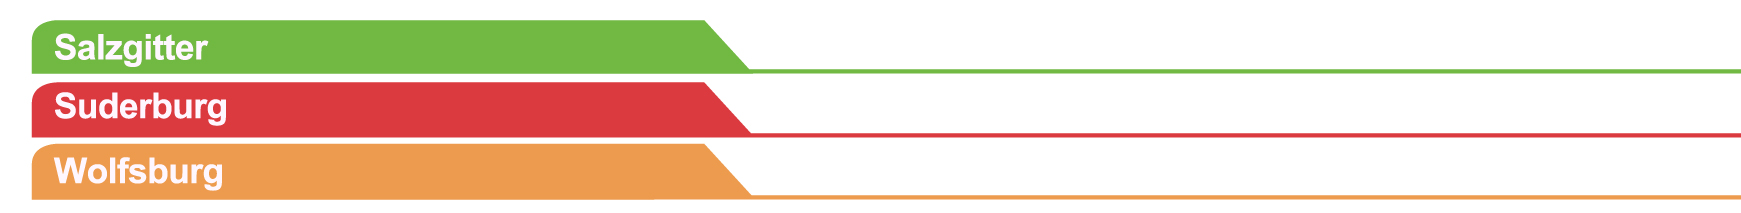
\includegraphics[scale=1.20]{Bilder/reiter_szsudwob_174mm.jpg}
	
	%*******************************************************************************
\end{titlepage}

\restoregeometry

	
	\tableofcontents
	\listoffigures
	\listoftables
	\pagebreak
	\thispagestyle{empty}
\chapter*{Abkürzungsverzeichnis}
\begin{acronym}[Bash]
    \acro{HZI}{Helmholtz Zentrum für Infektionsforschung}
    \acro{COVID-19}{Coronavirus SARS-CoV-2}
    \acro{SORMAS}{Surveillance, Outbreak Response Management and Analysis System}
    \acro{GA}{Gesundheitsamt}
    \acro{GAs}{Gesundheitsämter}
    \acro{SORMAS-ÖGD}{Sormas-ÖGD-Covid-19}
    \acro{VM}{Virtuelle Maschine}
    \acro{COP}{Container Orchestration Platform}
    \acro{OS}{Operating System}
    \acro{I/O}{input/output}
    \acro{OCI}{Open Container Initiative}
    \acro{runtime-spec}{Runtime Sepcification}
    \acro{image-spec}{Image Specification}
    \acro{CRI}{Container Runtime Interface}
    \acro{YAML}{YAML Ain't Markup Language}
    \acro{SSH}{Secure Shell}
    \acro{CNCF}{Cloud Native Computing Foundation}
    \acro{FOSS}{Free Open Source Software}
    \acro{OSF}{OpenStack Foundation}
    \acro{gRPC}{gRPC Remote Procedure Calls}
    \acro{DNS}{Dynamic Name Resolution}
    \acro{API}{Artificial Programming Interface}
    \acro{HTTP}{Hypertext Transfer Protocol}
    \acro{HTTPS}{Hypertext Transfer Protocol Secure}
    \acro{URL}{Uniform Resource Locator}
    \acro{SSL}{Secure Sockets Layer}
    \acro{TLS}{Transport Layer Security}
    \acro{PVC}{Persistent Volume Claim}
    \acro{PV}{Persistent Volume}
    \acro{NUC}{Next Level of Computing}
    \acro{PSU}{Power Supply Unit}
    \acro{PDU}{Power Distribution Unit}
    \acro{IP}{Internet Protocol}
    \acro{DHCP}{Dynamic Host Configuration Protocol}
    \acro{MAC}{Media Access Control}
    \acro{NAT}{Network Address Translation}
    \acro{KVM}{Kernel Virtual Machine}
    \acro{TOML}{Tom's Obvious, Minimal Language}
    \acro{regex}{regular expressions}
    \acro{TTL}{Time To Live}
    \acro{CNI}{Container Network Interface}
    \acro{CPU}{Central Processing Unit}
    \acro{S3}{Simple Storage Service}
    \acro{CRD}{Custom Resource Definition}
    \acro{DMZ}{demilitarized zone}
    \acro{GUI}{Graphical User Interface}
    \acro{DSGVO}{Datenschutz Grundverordnung}
\end{acronym}    


	\chapter*{Erklärung}

Hiermit versichere ich, dass ich die vorliegende Arbeit selbständig verfasst und keine anderen als die angegebenen Quellen und Hilfsmittel benutzt habe. Ich versichere, dass ich alle wörtlich oder sinngemäß aus anderen Werken übernommenen Aussagen als solche gekennzeichnet habe, und dass die eingereichte Arbeit weder vollständig noch in wesentlichen Teilen Gegenstand eines anderen Prüfungsverfahrens gewesen ist.

\vspace*{3em}

\newcommand*{\SignatureAndDate}[1]{
	\par\noindent\makebox[52mm]{\hrulefill}     \hfill\makebox[65mm]{\hrulefill}
	\par\noindent\makebox[52mm][l]{Ort, Datum}	\hfill\makebox[62mm][l]{#1}
}

\SignatureAndDate{Unterschrift}
	
	\mainmatter
	\chapter{Einleitung}

Die \ac{COVID-19} Pandemiesituation in Jahr 2020 stellte auf der ganzen Welt Gesundheitssysteme auf die Probe. 
Um das Virus bestmöglich bekämpfen zu können wurde das \ac{SORMAS}\footnote{2014 haben sich unter der Organisation des \ac{HZI} öffentliche Gesundheitsinstitutionen Deutschlands und Nigerias, sowie Forschungsinstitute und eine Software Entwicklungs Firma zusammengeschlossen um das Produkt \ac{SORMAS} zu entwickeln.
Die Software hatte den Zweck, den Ebola Ausbruch in Westafrika 2014/2015 einzudämmen.
In ihr können Fälle erfasst und gemanagt werden, um so Infektionsketten zu durchbrechen.
2016 wurde die Applikation zu einer Open Source Software migriert um die Unabhängigkeit von IT Firmen zu garantieren.
\cite{SORMAS_history}} vom \ac{HZI}\footnote{Das \ac{HZI} ist eine vom Bund finanzierte Instanz, an der Wissenschaftler alle möglichen Aspekte von Infektionskrankheiten untersuchen:
Wie werden diese ausgelöst und übertragen?
Wie werden sie vom Körper bekämpft?
Welche Wirkstoffe können bei der Infektionsbekämpfung hilfreich sein?
Warum sind einige Menschen anfälliger für Infektionskrankheiten als andere?
Mithilfe der Beantwortung dieser Fragen sollen Infektionskrankheiten im der aktuellen Zeit besser verstanden und bekämpft oder präventioniert werden. 
\cite{HZI_about}
\\
Aufgrund der Ausrichtung des \ac{HZI} beschäftiget sich das Institut im Jahr 2020 mit dem \ac{COVID-19}.} angepasst, um mit der Applikation nicht nur infizierte Personen managen zu können, sondern auch Kontaktpersonen zu erfassen.
Die neu entstandene Applikation bekam den Namen \ac{SORMAS-ÖGD} und wird vom Bund allen deutschen Gesundheitsämtern kostenlos zur Verfügung gestellt. 
\cite{SORMAS_covid}
\\
Deutschland hat insgesamt rund 400 \ac{GAs} \cite{GAs} von denen zum Zeitpunkt der Verfassung dieses Dokuments\footnote{07.10.2020} bereits 53 mit \ac{SORMAS-ÖGD} ausgestattet sind.
Diese Zahl nimmt jedoch stetig zu.  
An dieser Stelle kommt die Firma Netzlink~\ref{app:netzlink} ins Spiel: 
Die Firma hat durch eine Ausschreibung einen Vertrag mit dem Bund abgeschlossen, nach dem Netzlink jedem \ac{GA}, das interessiert ist, eine \ac{SORMAS-ÖGD}-Instanz zur Verfügung stellt.

\section{IST-Zustand}
Aktuell stellt Netzlink die \ac{SORMAS}-Instanzen auf ihrer VMWare\footnote{https://www.vmware.com/}-Infrastruktur zur Verfügung. 
\\
Die Daten, die in der \ac{SORMAS}-Datenbank gespeichert werden sind sogenannte besonders schützenswerte Daten.
\begin{quote}
    Bei Gesundheitsdaten gelten jedoch weitaus strengere Regeln als bei einfachen personenbezogenen Daten. 
    Gesundheitsdaten sind sensible, besonders schützenswerte Daten und werden im Gesetz als „besondere Kategorie“ personenbezogener Daten behandelt. 
    Grundsätzlich ist es untersagt, Gesundheitsdaten zu verarbeiten. 
    Dieses Verbot gilt nur dann nicht, wenn einer der gesetzlich geregelten Ausnahmefälle gegeben ist (Artikel 9 Abs. 2–4 \ac{DSGVO}). 
    \cite{Gesundheitsdatenschutz}
\end{quote}
Für die Netzlink als Provider der Applikation bedeutet das, dass die Daten der einzelnen \ac{GAs} streng getrennt werden müssen. 
Es dürfen nicht zwei Instanzen von \ac{SORMAS-ÖGD} auf der selben Maschine gehostet werden, da durch das Ausnutzen von Sicherheitslücken eventuell ein \ac{GA} die Daten eines Anderen einsehen könnte.
Um diese Abgrenzung zu garantieren rollt Netzlink mithilfe von Ansible\footnote{https://www.ansible.com/} für jedes \ac{GA} eine eigene \ac{VM} aus, um die Datensicherheit zu gewährleisten.
Auf der jeweiligen \ac{VM} werden dann mittels Docker \footnote{https://www.docker.com/} mehrere Container gestartet, die gemeinsam die \ac{SORMAS-ÖGD} Applikation darstellen.
\\
Für jedes \ac{GA} eine eigene VM zu bauen verbraucht unnötig viele Ressourcen:
\begin{itemize}
    \item Arbeitsspeicher für den Overhead der \ac{VM}
    \item Arbeitsspeicher und CPU Ressourcen um das Betriebssystem auf der \ac{VM} zu betreiben
    \item Zeit um die \ac{VM} auszurollen und zu starten 
\end{itemize}

\section{SOLL-Zustand}
Die ressourcenschonendere Lösung wäre, eine Containerplattform wie Kubernetes\footnote{https://kubernetes.io/} zu nutzen.
So kann viel Overhead eingespart werden, die Applikation kann schneller und zuverlässiger bereitgestellt werden. 
Die Abgrenzung, und damit der Schutz der Daten muss dabei unbedingt bestehen bleiben.

\section{Problemstellung}
Um den Schutz der besonders schützenswerten Daten zu garantieren muss eine Isolation geschaffen werden, die normalerweise bei einer Containerplattform nicht gegeben ist. 
Die Datenbank der verschiedenen \ac{GAs} dürfen nicht auf einer Maschine, also auf einem Kernel, laufen.
Diese Bedingungen können mit der Container Runtime "Kata-Containers"\footnote{https://katacontainers.io/} erfüllt werden. 
Die Funktionsweise dieser Runtime wird im Verlauf der Arbeit ausführlich erklärt. 
An dieser Stelle sei nur schon einmal vorweggenommen, dass diese Runtime die Prinzipien von \ac{VM}s und Containern  verbindet. 
Die "Container" die in dieser Runtime gestartet werden bekommen einen eigenen Kernel und sind daher eigentlich kleine \ac{VM}s, die sich jedoch wie Container anfühlen und bedienen lassen.
Hierbei wurde darauf geachtet, dass der Overhead der Instanzen so klein wie möglich gehalten wird, um das Container-Verhalten zu ermöglichen.
Die Aufgabenstellung ist also, eine Containerplattform aufzubauen die kata als Runtime nutzen kann.
Anschließend soll das bestehende \ac{SORMAS} mit seiner vollen Funktionalität auf Kubernetes migriert werden.

\section{Aufbau der Arbeit}
In Kapitel 2 werden die technischen Grundlagen, auf denen dieses Projekt aufbaut, erklärt. 
Hierbei wird kurz die Funktionsweise von Kubernetes angerissen, um die Integration von Kata-Containers in Kubernetes nachvollziehen zu können.
Die Unterschiede zwischen \ac{VM}s und und Containern werden herausgearbeitet und die Prinzipien der Kata-Runtime erklärt.
\\
Im Kapitel 3 wird der Aufbau und die Konfiguration des Clusters behandelt, dieses gliedert sich in:
\begin{itemize}
    \item Hardware Konfiguration
    \item Vorbereitung des Maschinen
    \item Netzwerk-Konfiguration
    \item Installation und Konfiguration von Kata
    \item Installation eines Kubernetes-Clusters
\end{itemize}

Kapitel 4 behandelt die Migration der \ac{SORMAS}-Applikation.
\ac{SORMAS} besteht aus einem Webserver, einer Autoheal-Funktion, einem Backup, einer Java Anwendung auf einem Payara-Server und einer Postgres-Datenbank.
Jeder dieser Teile muss auf der \ac{COP} abgebildet werden.
\\
Nach der Fertigstellung, in Kapitel 5, wird ein Fazit über das Projekts gezogen, und anschließend im letzten Kapitel 6 wird ein Ausblick auf den Verlauf des Projekts sowie zusätzliche Anwendungsmöglichkeiten gegeben.

	\chapter{Grundlagen: VMs, Container, Laufzeiten und Kubernetes}

\section{Virtuelle Maschinen} 
Die hier gesammelten Informationen wurden bei IBM\cite{vm} recherchiert. IBM ist mit RedHat ein Vorreiter auf diesem Bereich.\\
Als virtuelle Maschine bezeichnet man die Emulation einer physischen Maschine.
Durch Virtualisierung ist es möglich mehrere dieser \ac{VM}s auf einer Hardwaremaschine laufen zu lassen.
So können Maschinen mit verschiedenen Hardware-Eigenschaften, Betriebssystemen und Applikationen sich die zur Verfügung stehenden Ressourcen teilen, so dass sparsamer gearbeitet werden kann.

\subsection{Wie Virtualisierung funktioniert}
Eine \ac{VM} kann nicht direkt mit der ihr zugrunde liegenden Hardware kommunizieren. 
Sie benötigt dafür einen sogenannten Hypervisor.
Der Hypervisor ist eine dünne Softwareschicht, die auf dem Host läuft, und über die physische Ressourcen den einzelnen \ac{VM}s zugewiesen werden können.

Hypervisor lassen sich in zwei Typen einordnen:
\begin{itemize}
    \item Typ 1 \\ 
            Der Hypervisor wird direkt auf dem bare metal Server installiert, womit eine geringe Latenz und hohe Sicherheit garantiert werden.
    \item Typ 2\\
            Zwischen dem bare metal Server und dem Hypervisor ist eine \ac{OS} Schicht installiert. 
            Dieser Typ findet hauptsächlich bei Endnutzern Verwendung, die auf ihrer lokalen Maschine Virtualisierung betreiben wollen, zum Beispiel um eine \ac{VM} zu testen bevor sie auf der eigentlichen Virtualisierungsumgebung ausgerollt wird.
            Durch die zusätzliche \ac{OS} Schicht ist die Latenz höher als beim ersten Typen.
\end{itemize}

Durch die Unabhängigkeit von der Hardware ist es möglich die \ac{VM}s problemlos zwischen verschiedenen Hosts zu verschieben. \\

\subsection{Vorteile von Virtuellen Maschinen}
Da sich durch diese Technologie mehrere Applikationen und Maschinen dieselben Ressourcen teilen können, ist das Arbeiten mit \ac{VM}s deutlich ressourcenschonender und effizienter als das Arbeiten mit klassischen Hardware-Servern.
Durch den geringeren Verbrauch von Mitteln zahlt sich das Einsetzen auch aus finanzieller Sicht aus.
Des weiteren können die Server deutlich agiler gemanagt und vor allem auch schneller bereitgestellt werden.
Die Agilität führt auch dazu, dass Downtimes bei Umzügen oder Updates der Umgebungen reduziert werden.



\section{Container}
Die Informationen aus diesem Absatz stammen von Google\cite{containers}, einem der größten Innovatoren auf dem Bereich der Containertechnologien.
\subsection{Was ist ein Container?}
Unter einem Container verstehen wir ein vollständiges Paket, dass alle Bausteine enthält um eine bestimmt Applikation zu deployen.
Da alle Bestandteile in Ihm vereint sind ist das Deployment der Anwendung so komplett unabhängig von der zugrundeliegenden Umgebung, was den Prozess vereinfacht und zuverlässiger macht.
Außerdem erlaubt es diese Isolierung der Applikation auch eine klare Grenze zwischen Anwendungsentwickler und Betrieb zu ziehen:
Der Entwickler kann sich darauf verlassen, dass seine Software immer unter den exakt gleichen Bedingungen ausgeführt wird, mit den gleichen Abhängigkeiten, den gleichen Software-Versionen und auf dem gleichen Betriebssystem.
\\
Der IT-Betrieb hingegen kann sich darauf verlassen, dass ein Container sich immer gleich verhält. 
Er muss für verschiedene Anwendungen keine unterschiedlichen Betriebssysteme und Software-Versionen installieren, sondern muss nur den Container managen.
\\
Container können also, wie auch \ac{VM}s, als isolierte Umgebungen betrachtet werden, sie sind allerdings deutlich kleiner.

\subsection{Vorteile von Containern}

Container virtualisieren auf \ac{OS}-Level und auf dem gleichen Kernel wie das \ac{OS}.
Dadurch können sie deutlich schneller gestartet werden und haben einen deutlich kleineren Overhead als \ac{VM}s, da sie kein komplett funktionsfähiges Betriebssystem benötigen um zu laufen.
Der komplette Speicherplatz-, \ac{CPU}- und Arbeitsspeicher-Verbrauch des \ac{OS} wird somit an Ressourcen auf dem Host-System eingespart.

\subsubsection{Gleichbleibende Umgebung}
Da in dem Container immer von einer gleichbleibenden Umgebung ausgegangen werden kann, wird die Produktivität der einzelnen Entwicklern deutlich gesteigert.
Diese müssen sich, durch die Verwendung von Container-Technologien, nicht länger mit unterschiedlichen Umgebungsbedingungen auseinandersetzen und können sich auf das Entwickeln neuer Featuren konzentrieren.

\subsubsection{Auf jeden System ausführbar}
Container sind auf fast jedem System ausführbar. 
Ob Linux, Mac, Windows, \ac{VM}s, Datacenter oder Bare Metal.
Dies wird nicht zuletzt durch das sehr populäre Docker Image Format gewährleistet, das überall sehr verbreitet ist. 

\subsubsection{Isolation}
Arbeitsspeicher, \ac{CPU} und Speicher sind auf Betriebssystemebene virtualisiert und somit bis zu einem gewissen Level vom Rest des Systems abgegrenzt.
Die Isolation ist jedoch weniger stark als bei \ac{VM}s.



\section{Vergleich von Virtuellen Maschinen und Containern}

Beide Technologien haben ähnliche Ziele: \\
Höhere Schnelligkeit und Agilität beim Bereitstellen von Software, geringere Downtimes und Einspraung von Ressourcen. \\
Durch die unterschiedliche Herangehensweise hat jede Technologie andere Anwendungsbereiche als Ziel, sowie andere Stärken.
Die zusätzliche \ac{OS}-Schicht, in Abbildung \ref{fig:comparison_vm_container} dargestellt, bringt zwar einen deutlich größeren Overhead mit sich, dafür aber auch bessere abgrenzen der einzelnen Applikationen voneinander.
Die wichtigsten Unterschiede sind in Tabelle \ref{table:comparison_vm_container} noch einmal zusammengefasst. 

\begin{table}[ht]
        \centering
        \begin{tabular}{ | p{0.25\textwidth} | p{0.25\textwidth} | p{0.25\textwidth} | }
        Kategorie & Virtuelle Maschine & Container \\
        \hline \\
        Startup-Zeit & Im Minuten Bereich & Millisekunden bis Sekunden \\
        Performance & Großer Overhead, dadurch reltiv langsam & Kleiner Overhead, sehr schnell\\
        Operating System & Jede \ac{VM} kann auf einem unterschiedlichen \ac{OS} laufen & Alle Container teilen sich das \ac{OS} des Hosts \\
        Operations & Anpassungen müssen auf den \ac{VM}s vorgenommen werden. Unterschiedliche Maschinen, welche dieselbe Applikation bereitstellen können sich somit trotzdem unterscheiden. & Durch die deklarative Natur der Containertechnologien müssen keine Administratoren den Containern arbeiten. Anpassungen werden ausschließlich in den Images und Dockerfiles vorgenommen. Der Administrative Aufwand ist sehr gering. \\
        \end{tabular}
        \caption{Unterschiede von VM's und Containers}
        \label{table:comparison_vm_container}
\end{table}
\todo{Isolation hinzufügen}


\begin{figure}[ht]
        \caption{Vergleich von Virtuellen Maschinen und Containern\cite{vm_vs_container}}
        \centering
        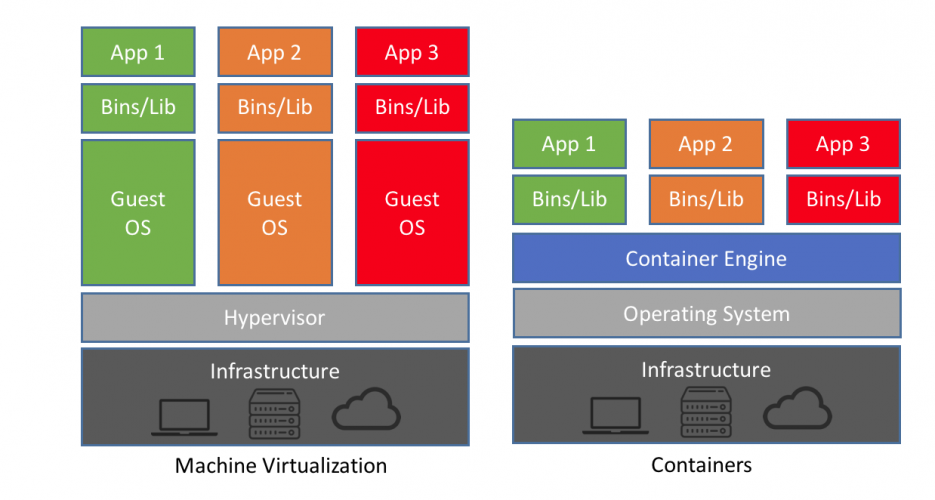
\includegraphics[width=0.8\textwidth]{bilder/comparison_vm_container.png}
        \label{fig:comparison_vm_container}
\end{figure}



\section{Open Container Initiative}
Die \ac{OCI} ist eine Organisation, die Standards für Container Runtimes und Formate erstellt.
Aktuell werden zwei Spezifikationen von der Organisation bereitgestellt, die \ac{runtime-spec} und die \ac{image-spec}.
Die Spezifikationen erlauben es verschiedener Software, das bereitgestellt Interface zu implementieren.
Die \ac{runtime-spec} definiert wie ein Container auf dem Host ausgeführt werden muss. 
Eine \ac{OCI}-Implementation, wie zum Beispiel Docker, lädt zum Ausführen eines Containers ein \ac{OCI}-kompatibles Container-Image herunter und entpackt dieses in ein Runtime Filesystem Bundle.
Ohne die Definitionen des \ac{OCI} könnte ein Container der im Docker-Format und die Docker-Runtime(\texttt{runc}) geschrieben wurde auch nur von Docker ausgeführt werden.
Die \ac{OCI}-Spezifikation ermöglicht es, mit jeder Container-Runtime, die \ac{OCI}-kompatibel ist, ein Docker-Image auszuführen. \cite{oci}



\section{Kubernetes}
Kubernetes ist eine \ac{FOSS}-Lösung zum managen von containerisierten Anwendungen.
Das System ermöglicht automatisches Skalieren und Deployen der Anwendungen, sowie integriertes Self-Healing, einfaches Management und Updaten.
Außerdem ist es vergleichsweise unproblematisch ein Kubernetes-Cluster selbst zu skalieren. 
Nodes lassen sich im Live-Betrieb nicht nur hinzufügen, sondern können genauso auch ausfallen. 
Die auf ihnen laufenden Container werden dann, wenn möglich ohne Downtimes, auf die verbliebenen zur Verfügung stehenden Nodes verteilt. 
Gehostet werden kann Kubernetes sowohl on-premise als auch in der public- oder hybrid-cloud.
\\
Entwickelt wurde die Technologie ursprünglich von Google, die schon seit 15 Jahren Produktions-Arbeitslast in Containern laufen lassen.
\cite{kubernetes}

\subsection{Cluster Komponenten}
\subsubsection{Proxy}
Der Proxy ist dafür verantwortlich, den Netzwerk-Verkehr zu Services in dem Kubernetes-Cluster zu routen. 
Dafür muss auf jeder Maschine des Clustern der entsprechende Proxy vorhanden sein, was mit der Kubernetes-Ressource \textit{DaemonSet} realisiert werden kann.
Diese sorgt dafür, dass auf jedem Node des Clusters der entsprechende Container läuft.\cite[S.34]{Kubernetes_up_and_running}
\subsubsection{DNS}
Der \ac{DNS}-Server ist für die Namensaulösung und die Entdeckung von Services innerhalb des Clusters verantwortlich. 
Der \ac{DNS}-Server selbst läuft als ein eigener Service in dem Cluster.
Damit er funktionieren kann, muss da Cluster mit einem funktionieren Container-Network ausgestattet sein. 
\cite[S.34 f]{Kubernetes_up_and_running}

\subsection{Container Runtime Interface}
In Kubernetes 1.5 wurde in Kubernetes das \ac{CRI} eingeführt.
Dieses Interface erlaubt es dem \texttt{kubelet} mit jeder Container Runtime zu arbeiten, die selbst dieses Interface implementiert. 
\texttt{Kubelet} kommuniziert über einen \texttt{shim} mit der Runtime, wobei der \texttt{shim} als Server funktioniert und \texttt{kubelet} als Client.
Der \texttt{\ac{CRI} shim} gibt dann die Befehle an die Runtime weiter, wie in Abbildung \ref{fig:cri} dargestellt.
\begin{figure}[ht]
        \caption{Kubernetes \ac{CRI}\cite{kubernetes_cri}}
        \centering
        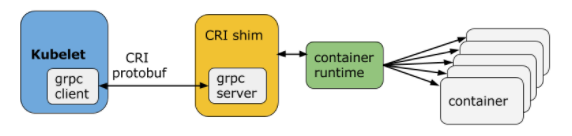
\includegraphics[width=\textwidth]{bilder/kubernetes_cri.png}
        \label{fig:cri}
\end{figure}
\cite{kubernetes_cri}

\subsection{Pods}
Ein Pod ist der kleinste Workload in einem Kubernetes Cluster, in ihm können ein oder mehrere Container laufen.
Wenn ein Pod-Manifest an die Kubernetes-\ac{API} geschickt wird, entscheidet der \texttt{sheduler} auf welchem der Nodes der Pod gestartet werden soll.
Gestartet und am Leben erhalten wird der Pod dann vom \textit{kubelet daemon}.
\cite[S.63]{Kubernetes_up_and_running}

\subsection{Service}
Das Service Objekt in Kubernetes wird benötigt um einen Service inner- oder außerhalb des Clusters zu exposen.
Services werden benötigt um verlässlich auf einen Pod zugreifen zu können.
Da sich in Kubernetes die Namen der einzelnen Pods bei jedem Neustart ändern können, wird ein gleichbleibendes Objekt benötigt, über das immer dieselbe dahinterliegende Applikation erreicht werden kann.
Diese Rolle übernimmt der Service.
Über Labels werden sie mit einzelnen Pods verknüpft und macht diesen so, über den Service, erreichbar.
\cite[S.86]{Kubernetes_up_and_running}

\subsection{Ingress}
Der Ingress leitet von \ac{HTTP} und \ac{HTTPS} Routes auf Services innerhalb des Clusters weiter.
Mithilfe dieser Ressource können Services mit \ac{URL}'s verknüpft werden, Load kann verteilt werden und \ac{SSL} / \ac{TLS} terminiert.
Beispielsweise können so \ac{URL}'s wie \textit{service1.host.com} und \textit{service2.host.com} zu den entsprechenden Services und Ports auf dem gleichen Host gemappt werden, wie in Abbildung \ref{fig:ingress} dargestellt.
\cite{kubernetes_ingress}
\begin{figure}[ht]
        \caption{Kubernetes Ingress\cite{kubernetes_ingress}}
        \centering
        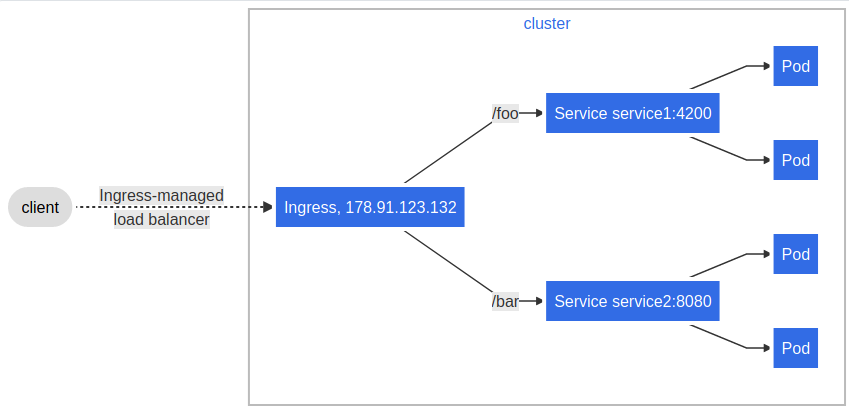
\includegraphics[width=\textwidth]{bilder/kubernetes_ingress.png}
        \label{fig:ingress}
\end{figure}

\subsection{Replica Set}
Ein Replica Set lässt sich als Pod-Manager beschreiben. 
In dieser Ressource kann definiert werden, wie viele Kopien von welchem speziellen Pod vorhanden sein sollen.
Das Replica Set wird dann immer dafür sorgen, dass genau so viele Kopien des Pods auf dem Cluster laufen wie deklariert. 
Wenn ein oder mehrere Pods sterben, die von einem Replica Set gemanagt werden, werden diese automatisch erneut gestartet. 
So lange bis wieder die gewünschte Anzahl an Pods erreicht ist.
Selbst wenn ein kompletter Node ausfällt, kümmert das Replica Set sich darum, dass der Pod auf einem anderen Node gestartet wird.
\cite[S.103 ff.]{Kubernetes_up_and_running}

\subsection{Deployment}
Das Deployment ist vor allem zum managen von neuen Software Releases gedacht. 
Durch den Rollout-Prozess wird es vereinfacht von einer Version der Software zur nächsten zu wechseln, zum Beispiel durch eingebaute Health-Checks die das Update anhalten wenn zu viele Instanzen der neuen Software-Version in einem Failed-State landen.
Durch Deployments können Downtimes komplett vermieden werden, indem von einer zu updatenden Software nach und nach die einzelnen Container durch Container mit der neuen Software Version ersetzt werden.
Wenn der letzte Container mit der alten Software-Version ersetzt wurde, ist das Update der Anwendungen ohne eine einzige Sekunde Downtime durchgeführt wurden.
Ein Deployment managt dazu Replica Sets, so wie diese die einzelnen Pods managen.
\cite[S.113 ff.]{Kubernetes_up_and_running}

\subsection{Stateful Set}
Stateful Sets sind ähnlich zu Replica Sets, haben aber einzigartige und eindeutige Eigenschaften.
Jede Kopie bekommt dazu einen persistenten Hostname, bei dem von 0 aufwärst hochgezählt wird. 
Wird das Stateful Set gelöscht, werden die Pods vom höchsten zum niedrigsten hin wieder gelöscht.
Durch den persistenten Namen ist es für andere Applikationen innerhalb des Clusters möglich immer genau die gleiche Instanz anzusprechen.
\cite[S.186 f.]{Kubernetes_up_and_running}

\subsection{Config Maps}
Eine ConfigMap wird genutzt um Konfigurations-Werte für eine Anwendungen zu setzen. 
Die gesetzen Variablen können das Environment das Containers definieren, mit dem sie verknüpft werden.
\cite[S.153]{Kubernetes_up_and_running}

\subsection{Secret}
Secrets sind sehr ähnlich zu Config Maps, mit dem einzigen Unterschied, dass die in ihnen gespeicherten Daten sensibel und deswegen verschlüsselt sind.
Das bedeutet, dass Sie sich für Passwörter, Security Token und secret Keys besser eigenen als Config Maps.
\cite[S.157 f.]{Kubernetes_up_and_running}

\subsection{Persistenter Storage}
Persistenter Storage in Kubernetes ist standartmäßig nicht gegeben. 
Die Plattform rechnet damit, dass die einzelnen auf ihr gehosteten Pods regelmäßig ausgetauscht zerstört werden. 
Um in so einem Umfeld persistenten Storage garantieren zu können gibt es in Kubernetes \ac{PV}s und \ac{PVC}s.

\subsubsection{Persistent Volume}
Ein \ac{PV} ist ein definierter Storage-Teil das mit einer Storage Class provisioniert wurde.
Ihr Lifecycle ist unabhängig von dem individuellen Pod der das \ac{PV} benutzt.

\subsubsection{Persistent Volume Claim}
Ein \ac{PVC} ist eine Anfrage des Users nach Storage.
In Ihnen werden Größe und Zugriffsart des benötigten Speicherplatzes definiert. 


\section{Kata-Runtime}
Das Kata Containers Projekt ist ein Open Source Projekt, das probiert die Vorteile beider zuvor erläuterten Technologien zu kombinieren.
Die Isolation von \ac{VM}s mit der Geschwindigkeit, dem geringen Management Aufwand und dem Self-Healing von Containern.
\\
Wenn ein Container-Image in der Kata-Runtime gestartet wird, wird tatsächlich kein Container gestartet, sondern eine lightweight \ac{VM} erstellt.
Diese hat ihren eigenen Kernel, der eine Isolation des Netzwerks, des Speichers und von \ac{I/O} garantiert, jedoch mit einem deutlich kleineren Overhead als konventionelle \ac{VM}s.
Um einen möglichst großen Anwenderbereich abzudecken arbeitet Kata nach den industriellen Standards \ac{OCI} und implementiert Kubernetes \ac{CRI}, das im Verlauf der Arbeit noch genauer geklärt wird. 
Durch die standardisierten Interfaces ist der Umstieg und das Arbeiten mit Kata in der Theorie sehr unkompliziert. \cite{kata}

\subsection{Geschichte}
Das Kata-Container Projekt entstand aus der Fusion von zwei vorhergehenden Projekten:
\begin{itemize}
        \item Clear Containers
        \\Dieses Projekt von Intel\footnote{https://www.intel.com/content/www/us/en/homepage.html} wurde 2015 ins Leben gerufen, um Sicherheitsbedenken beim Einsatz von Containern aus dem Weg zu räumen.
        Intel erschuf eine alternative Container Runtime, in der Container als minimale \ac{VM}s gestartet wurden, den Fokus setzten sie dabei auf Performance(<100ms boot time) und Sicherheit.\cite[S.1]{Kata_Containers}
        \item runV
        \\Ist ein ähnliches Projekt von der Firma "Hyper", die selbst eine Runtime entwickelt haben, die einen Hypervisor nutzt.
        Sie haben Ihren Fokus auf den Support vieler \ac{CPU}-Architekturen und Hypervisor gelegt.\cite[S.1]{Kata_Containers}
\end{itemize}
2016 hielten beide Firmen eine Präsentation über ihr jeweiliges Produkt auf der \say{Open Source Summit} in Berlin und wurden so aufeinander aufmerksam.
Ein Jahr später, in 2017, wurde beide Produkte unter der \ac{OSF} zu Kata-Containers zusammengeführt.\cite{kata_history}

\subsection{Vergleich mit traditionellen Containern}

\begin{figure}[ht]
        \caption{Vergleich von Kata-Containern und traditionellen Containern\cite{kata_learn}}
        \centering
        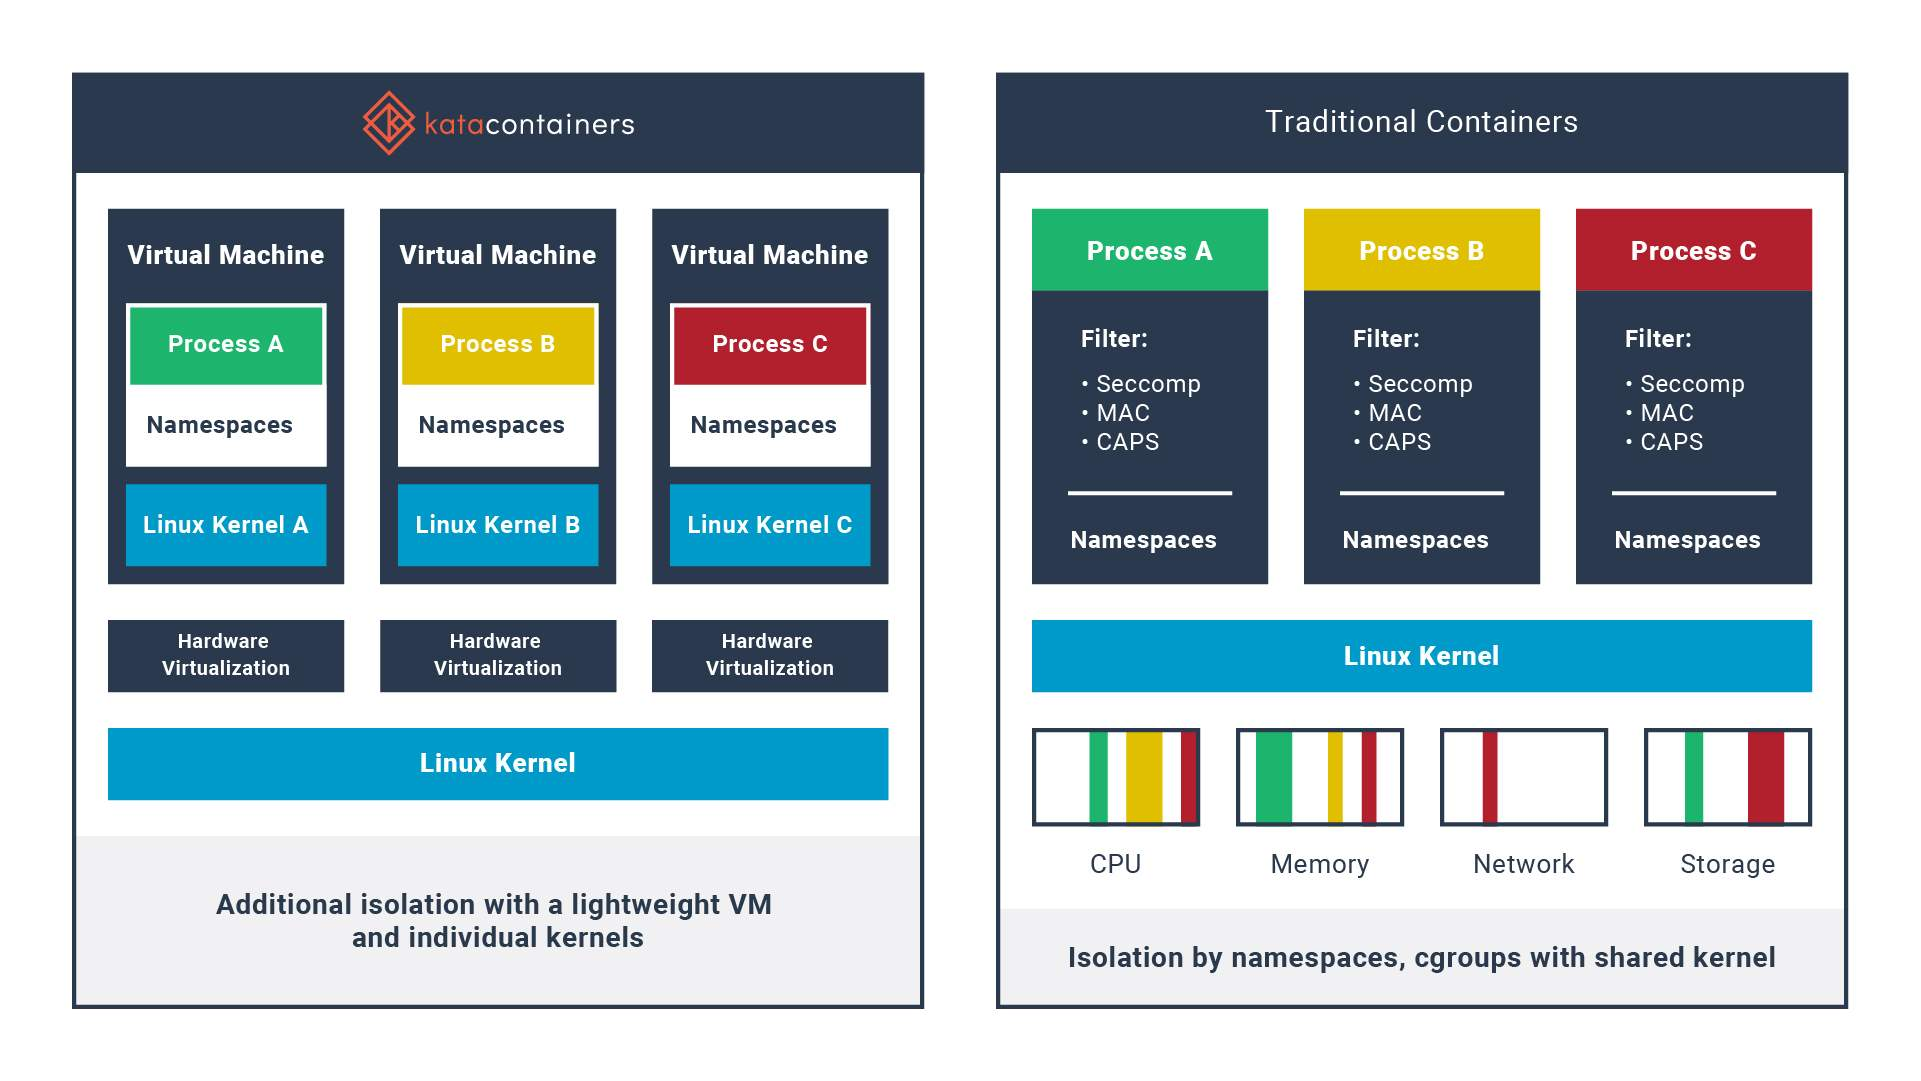
\includegraphics[width=\textwidth]{bilder/katacontainers_traditionalvskata_diagram.jpg}
        \label{fig:kata_vs_traditional}
\end{figure}

In der Abbildung \ref{fig:kata_vs_traditional} werden die wichtigsten Unterschiede dargestellt.
Traditionelle Container laufen alle auf demselben Kernel. 
Das bedeutet, dass jeder Container direkt auf den Ressourcen(\ac{CPU}, Memory, Network, Storage) des Hosts läuft. 
Eine Isolation wird durch Namespaces und cgroups realisiert.
\\
Bei den Kata-Containern hingegegen werden die Container in \ac{VM}s verpackt, von denen jede seinen eigenen Kernel bekommt.
Durch die Hardware-Virtualisierung kann jeder Container nur auf die Ressourcen zugreifen, welche für ihn erstellt wurden. 
In seinem Kernel laufen keine Prozesse, außer diejenigen der Applikation selbst.  

\subsection{Kata Container in Kubernetes}

\begin{figure}[ht]
        \centering
        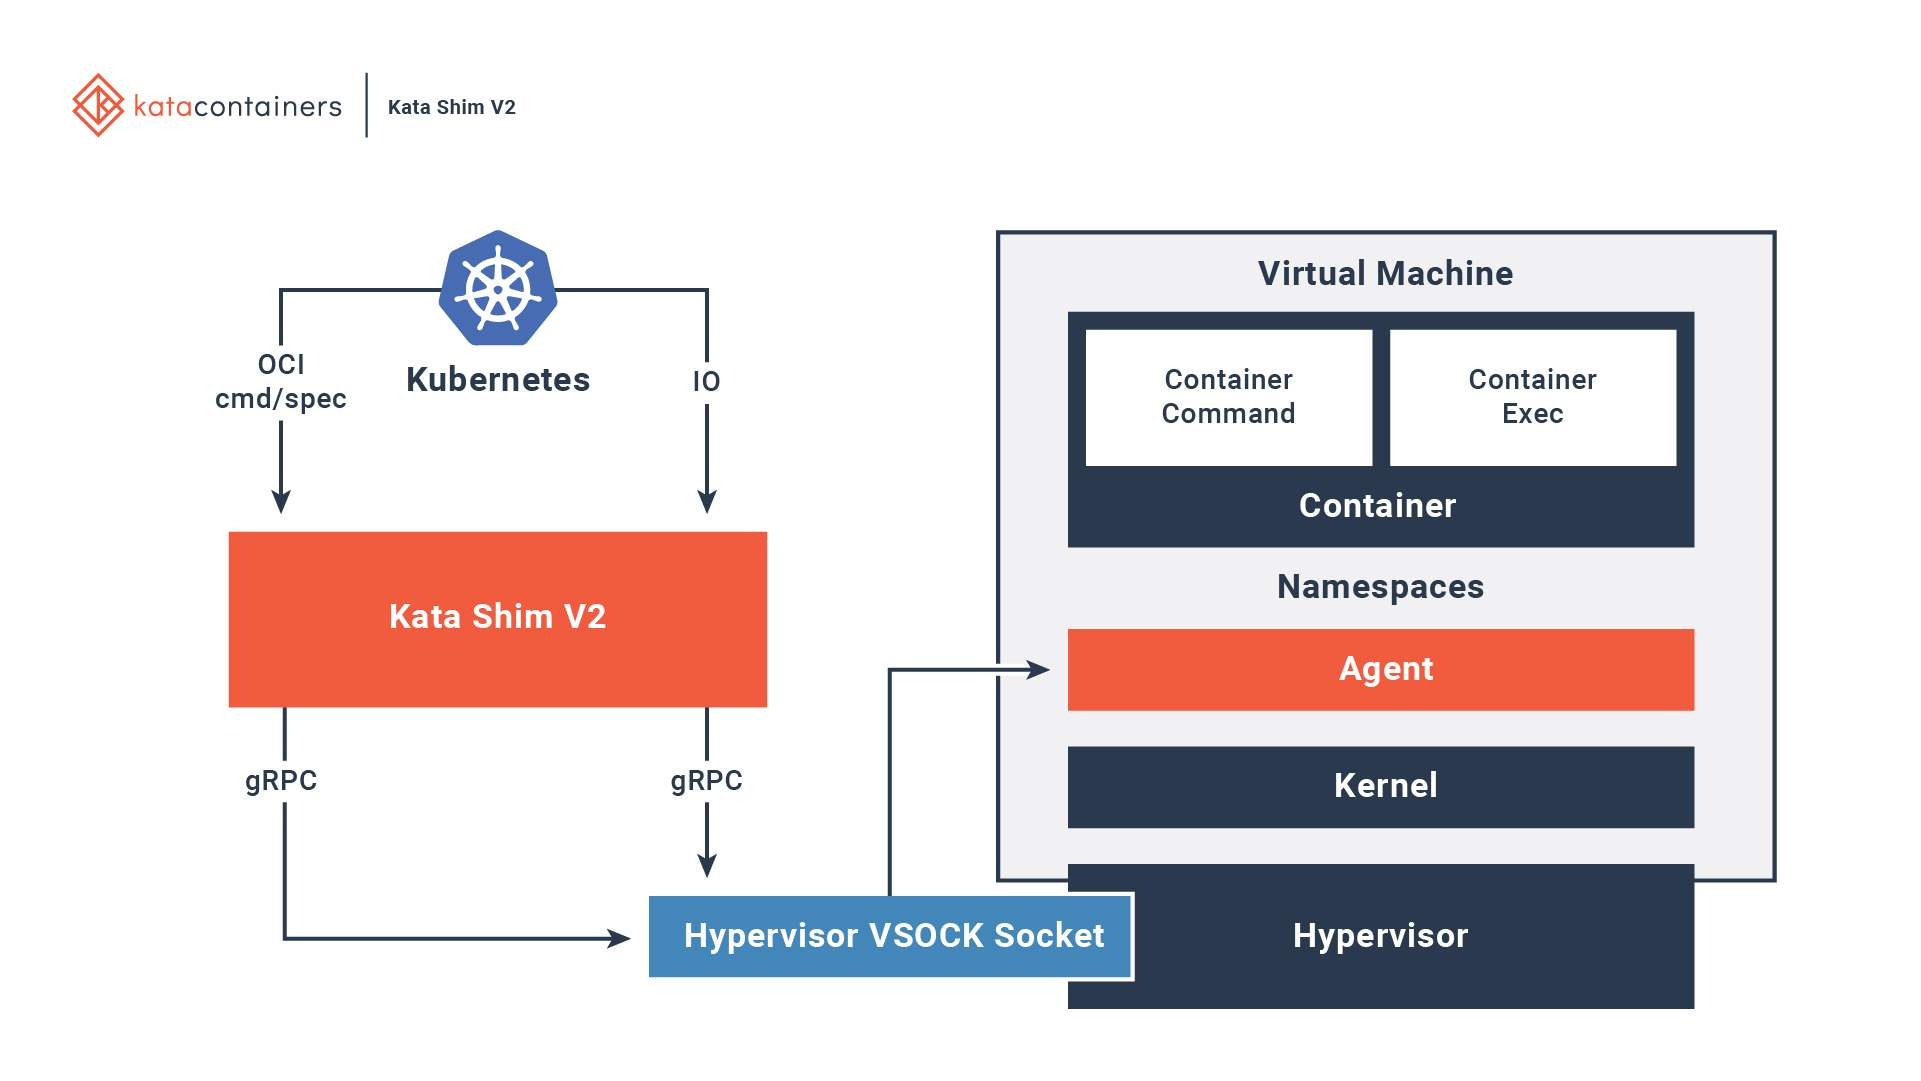
\includegraphics[width=\textwidth]{bilder/katacontainers_architecture_diagram.jpg}
        \caption{Kata Architektur\cite{kata_learn}}
        \label{fig:kata_architecture}
\end{figure}

In Abbildung \ref{fig:kata_architecture} lässt sich erkennen, dass eine Komponente namens \say{Kata Shim V2} eine große Rolle in der Kubernetes Integration spielt.
Kubernetes kann Pods und \ac{OCI}-kompatible Container mit dem \textit{kata-shimv2} starten. 
In der \ac{VM}, die von dem \textit{kata-shimv2} gestartet wurde, läuft unter anderem der \textit{kata-agent}, der für das Starten von Container-Prozessen eingesetzt wird.
Außerdem hostet er einen \ac{gRPC}-Server, über den der \textit{kata-shimv2} mit dem Agent in der \ac{VM} kommunizieren kann.
So können von dem Shimv2 Befehle zum managen von Containern in die Maschine gesendet werden, sowie \ac{I/O}-Streams transportiert werden, um so beispielsweise Commands in den Container auf dem Gast zu senden.
Auf diesem Weg werden aber genauso auch der \textit{stdout}- und \textit{stderr}-Stream an den \ac{CRI} Shim transportiert.
\cite{kata_architecture}

\todo{Kata mit Containerd in Kubernetes https://github.com/kata-containers/documentation/blob/master/how-to/containerd-kata.md}



\section{Ansible}
Ansible ist eine Software, mit dessen Hilfe Systeme deployed und gemanagt werden können. 
Dazu wird ein Prozess, der eigentlich händisch ausgeführt werden würde, in einem sogenannten Playbook abgebildet.
Dieses Playbook beschreibt der Reihe nach genau jede Bedingung die erfüllt sein muss, um den Prozess abzuschließen.
Durch die deklarative Natur von Ansible sind die Ergebnisse reproduzierbar und führen nur die Änderungen aus, die nötig sind.
Wird ein wiederkehrendes Problem einmal in einem Ansible-Playbook gelöst, kann dieses Playbook immer wieder Verwendung finden, wenn das Problem erneut auf einem ähnlichen System auftritt.
Ansible lässt sich auch einsetzen, um den Umgang mit bereits eingesetzten Technologien zu vereinfachen oder zu automatisieren.
\cite{ansible}

\subsection{Funktionsweise}
Ansible ermöglicht es, die gesamte Infrastruktur mitsamt all ihren Verbindungen zu beschreiben. 
So kann die ganze Umgebung, statt nur einzelne Systeme, auf einmal angepasst werden.
Dazu nutzt Ansible die bereits angesprochenen Playbooks, die in \ac{YAML} geschrieben sind, einer deklarativen und sehr simpel gestalteten Sprache.
\\
Wird ein Playbook ausgeführt stellt Ansible auf den einzelnen Systemen mithilfe von einigen Modulen den gewünschten Stand her, und löscht diese Module anschließend wieder. 
Um die Verbindungen zu den einzelnen Systemen herstellen zu können nutzt die Software standartmäßig \ac{SSH}-Keys, es sind allerdings auch andere Identity-Management Systeme wie z.B. Kerberos unterstützt.
Die Systeme selbst werden in den Inventory Files aufgelistet und können mit Gruppen und Variablen ausgestattet werden, um in einer Infrastruktur beispielsweise nur die Webserver oder nur die Datenbank-Server anzusprechen.
Wird ein OpenStack oder Ähnliches als Infrastruktur genutzt, kann sogar ein dynamisches Inventory generiert werden.
\cite{how_ansible_works}
\\
In diesem Projekt soll Ansible verwendet werden, um einen reproduzierbaren Weg zum installieren und konfigurieren der Kata-Runtime zu finden, sowie um das Kubernetes Cluster aufzubauen und zu managen. 


\section{Helm}
Helm ist eine Software, die das Installieren und Updaten von komplexen Kubernetes Applikationen vereinfachen soll.
Helm-Charts sind einfach zu erstellen, sie bieten eine gute Versionierung, lassen sich veröffentlichen und teilen, sowie templaten.
Das Projekt ist ein \ac{CNCF}-Projekt und wird von der Community gepflegt.
Charts beschreiben komplexe Applikationen und ermöglichen somit eine vereinfachte Installation von umfangreicher Software, außerdem sind diese einfach zu teilen und somit ein guter Weg um Software zu veröffentlichen.
\cite{helm}
\\
Für das \ac{SORMAS}-Projekt wird Helm jedoch auch vor allem wegen der guten Templating Möglichkeiten eingesetzt.
Verschiedene \ac{GAs} benötigen unterschiedliche Attribute, die alle über das Helm-Templating gesetzt werden könne.
So kann garantiert werden, dass nur an einer einzigen Stelle im Code jemals Anpassungen gemacht werden müssen, wenn eine neue \ac{SORMAS-ÖGD}-Instanz ausgerollt werden soll.
	\chapter{Aufbau und Konfiguration des Clusters}

Dieses Kapitel bildet die erste Hälfte des praktischen Teils der Projektarbeit.
Dieser behandelt den Aufbau der Hardware, die Netzwerk Konfiguration, sowie die Installation der Kata-Runtime und letztendlich den Aufbau eines Kubernetes Clusters.
Am Ende diese Kapitels soll alles für das sichere Deployment von Sormas auf Kata Vorbereitet sein.  

\section{Hardware}
Für das Projekt wurde folgende Hardware verwendet:
\begin{itemize}
    \item 1 Intel Atom \ac{NUC}
    \item 3 Lenovo Workstations 
    \item 1 Linksys Netzwerk-Switch
    \item 5 Ethernet Kabel
    \item 1 \ac{PDU}
    \item entsprechende \ac{PSU}s
\end{itemize}

Der einzelne Intel \ac{NUC} soll in dem Cluster die Rolle des Masters einnehmen.
Die Workstations werden als Worker eingesetzt.
Der Switch und die Ethernet Kabel werden genutzt um ein isoliertes Netzwerk aufzubauen, davon wird sich eine geringere Latenz und bessere Labor Bedingungen versprochen.
Mithilfe der \ac{PDU} und \ac{PSU}s wird das Cluster mit Strom versorgt. 
Eine Bestimmung der Hardware lässt sich Tabelle \ref{table:hardware} entnehmen, für eine detallierte Version siehe Anhang \ref{table:hw_detail}.

\begin{table}[h]
    \centering
    \begin{tabular}{ p{ 0.3\textwidth } | p{ 0.3\textwidth } p{ 0.3\textwidth } }
        x & \ac{NUC} & Workstations \\
        \hline \\
        CPU & Intel\textregistered Celeron\textregistered N2930 CPU@1.83GHz &  Intel\textregistered Core\texttrademark i3-7100 CPU@3.90GHz \\
        Cores & 4 & 4 \\
        Arbeitsspeicher & 8GB & 8GB \\
        Speicherplatz & 196GB & 240 GB \\
    \end{tabular}
    \caption{Hardware}
    \label{table:hardware}
\end{table}


\section{Vorbereitung der Maschinen}
Um die Maschinen vorzubereiten wurden bei jeder einzelnen der Storage komplett formatiert.
Anschließend wurde auf allen Maschinen Ubuntu 20.04 als \ac{OS} installiert.
Ubuntu wurde auf Empfehlungen aus dem Unternehmen gewählt, da einige schon gute Erfahrungen mit Kubernetes auf Ubuntu gesammelt haben und ein gutes Tiefewissen vorhaben ist.
\\
Für jede Maschine wurde dabei ein User und ein Passwort eingerichtet, sowie der \ac{SSH} Zugriff von Außerhalb freigeschaltet.
Der SSH-Zugriff wird benötigt um die Maschinen leichter zugänglich zu machen, aber vor allem, um Sie mit Ansibel managen zu können.


\section{Netzwerk Konfiguration}
Als nächstes muss ein Netzwerk-Zugang für die Maschinen eingerichtet werden.
Das Netzwerk soll so gut wie möglich von den Produktiv-Netzwerken bei Netzlink abgegrenzt sein.
Durch ein Subnet kann erreicht werden, dass die Netzwerk Performance erhöht wird und die Maschinen nicht von anderem Traffic beeinflusst werden können.
Dadurch können insgesamt reproduzierbarere Ergebnisse erzielt werden. 
\\
Für diese Projekt soll des Subnetz von dem Master-Node aufgespannt werden. 
Dadurch kann der Master auch an anderer Stelle einfach mit dem Netzwerk verbunden werden und das interne Netz bleibt unverändert.
Für den Master wurde also eine statische Netzlink-Interne \ac{IP}-Adresse angefragt um über diese Adresse auch die restlichen Nodes an das Netzwerk anzuschließen.
Zusätzlich erhält der Master eine interne \ac{IP}-Adresse über die er mit den Nodes kommunizieren kann.
Die gewählten Adressen lassen sich Tabelle \ref{table:katanetes_ips} entnehmmen.

\begin{table}
    \centering
    \begin{tabular}[h!]{ c | c c }
        x & Externe \ac{IP} & Interne \ac{IP} \\
        \hline
        k8smaster & 10.10.6.60 & 192.168.0.1 \\
        k8sworker1 & - & 192.168.0.11 \\
        k8sworker2 & - & 192.168.0.12 \\
        k8sworker3 & - & 192.168.0.13 \\
    \end{tabular}
    \caption{Cluster IPs}
    \label{table:katanetes_ips}
\end{table}

Das Netzwerk wurde so geplant, dass nur der Master-Node einen Internet-Zugriff beötigt.
Auf Ihm wurde ein \ac{DHCP}-Daemon so eingerichtet, dass dieser jedem der Worker basierend auf deren \ac{MAC}-Addressen die richtige IP zuordnet. 
Die Configuration für den \ac{DHCP}-Server findet sich im Anhang unter \ref{app:dhcp}. 

Um den Maschinen den Internet-Zugang zu ermöglichen muss als letztes \ac{NAT} auf dem Master Node konfiguriert werden.
Dafür muss \textbf{net.ipv4.ip\_forward=1} in die \textit{/etc/sysctl.conf} eingetragen werden und anschließend der Server rebootet.
Außerdem müssen die \textbf{iptables} Regeln angepasst werden, damit der Traffic auf dem internen Interface auf das externe Interface weitergeleitet wird. 
Das externe Interface ist das \textbf{enp4s0} und das Interne ist \textbf{enp3s0}.
Für das externe Interface, also \textbf{enp4s0} muss zunächst \textbf{POSTROUTING} und \textbf{MASQUERADE} eingerichtet werden. 
Dadurch werden die Pakete, die an diesem Interface ankommen, mit der IP des Masters maskiert und dann surch das public Interface gesendet. 

Anschließend müssen alle Pakete die an \textbf{enp3s0} geschickt werden auf \textbf{enp4s0} geforwarded werden, sowie die ankommenden Pakete auf \textbf{enp4s0} wieder über \textbf{enp3s0} zu den entsprechenden Maschienen.

Die genau Konfiguration ist im Anhang unter \ref{app:iptables} zu finden. 

In Ubuntu 20.04 wird nicht wie vielleicht bekannt mit der rc.local gearbeitet, sondern mit den Tools \textbf{iptables-persistent} und \textbf{iptables-save}.

Das entstandene Netzwerk wird in Abbildung \ref{fig:network_diagramm} dargestellt.

\begin{figure}[h]
    \centering
    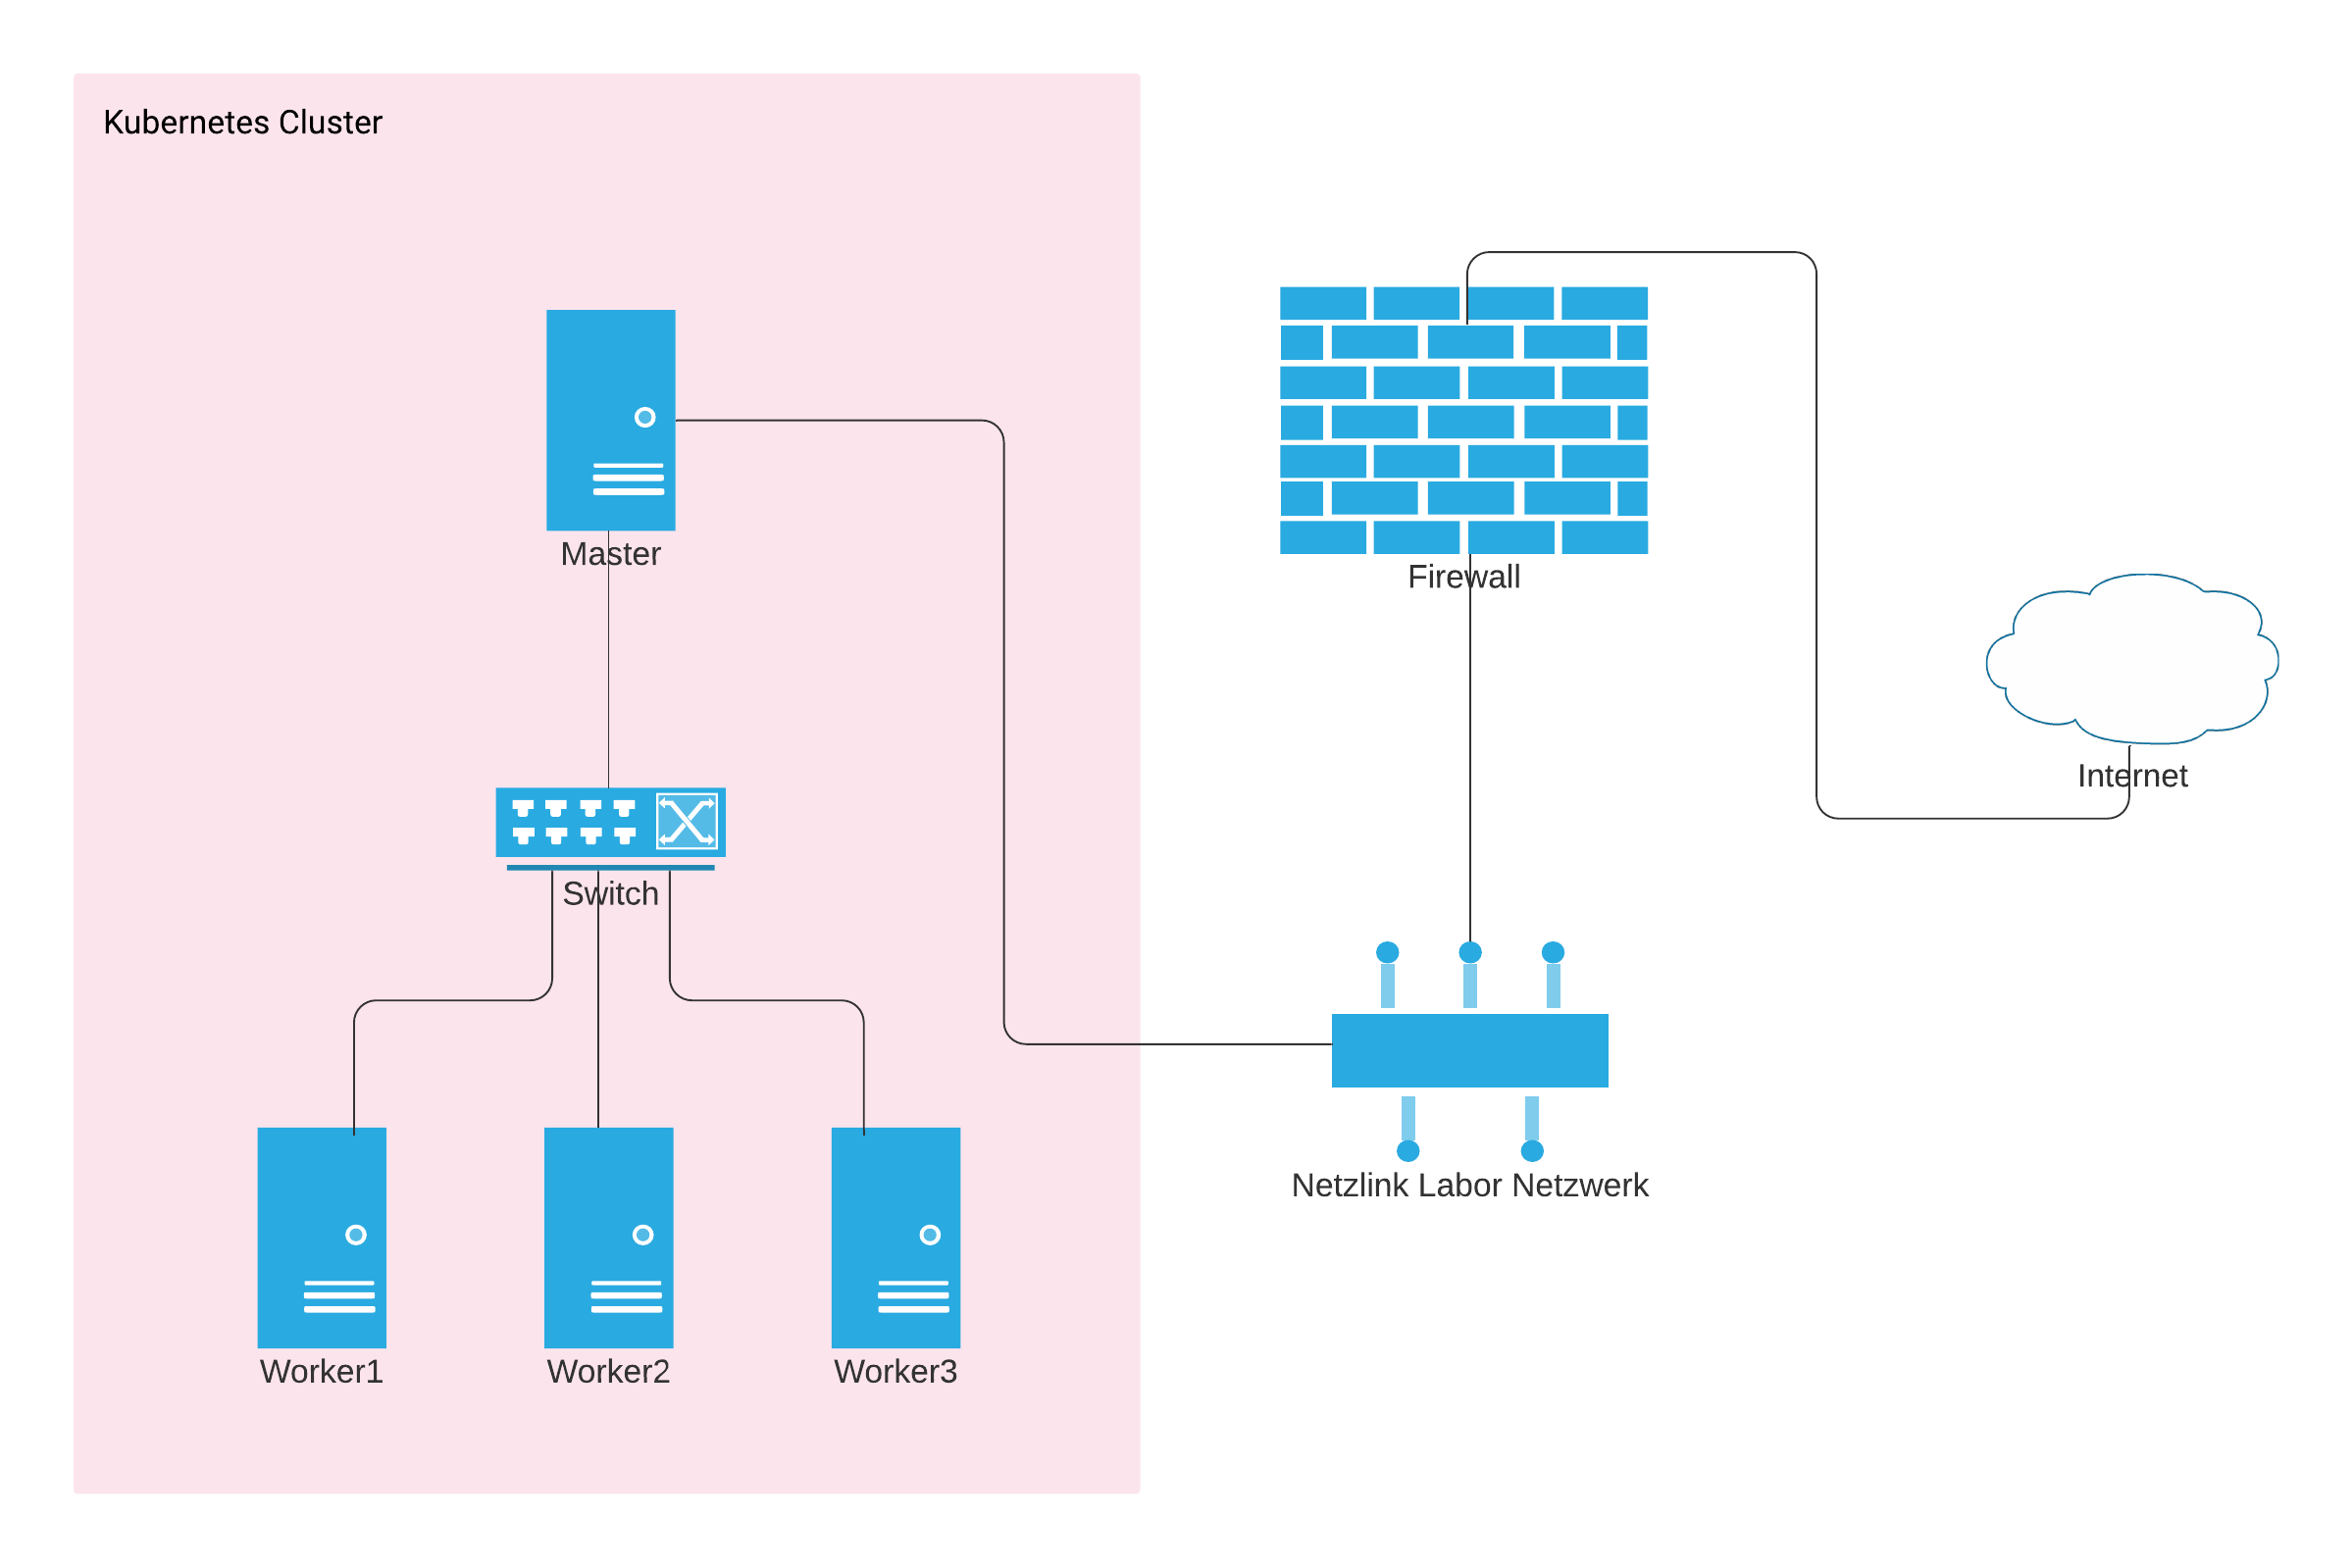
\includegraphics[width=\textwidth]{bilder/Katanetes Network.png}
    \caption{Netzwerkdiagramm}
    \label{fig:network_diagramm}
\end{figure}

\newpage

\section{Ansible Setup}
Von diesem Punkt an können nun alle Konfigurationen mit Ansible gemacht werden, da auf jeder der Maschinen \ac{SSH} konfiguriert ist und sie alle über eine Netzwerkverbindung verfügen.
Dazu muss nur auf dem Master Ansible installiert werden und der \ac{SSH} Zugang zu allen Zielsystemen konfiguriert sein. 
Für die Installation von Ansibel muss zunächst das Repository \textbf{ppa:ansible/ansible} zum Paketmanager hinzugefügt werden, dann können über \textbf{apt} die entsprechenden Pakete installiert werden.
Wie zuvor erwähnt muss die Ansibel Installation nur auf einer Maschine erfolgen.

Anschließend müssen für Ansible nur die Hosts, welche gemanaged werden sollem, in die \textit{hosts}-file eingetragen werden.
Dabei bietet Ansible die Möglichkeit Hostgruppen zu bilden. 
Wenn ein Playbok ausgeführt wird, kann die Hostgruppe angegeben werden, und alle Operationen werden dementsprechend auf alle Hosts in dieser Gruppe angewendet. 
Für dieses Projekt wurden die Gruppen \textbf{master} und \textbf{woker} gebildet.
Das Inventory kann im Anhang unter \ref{app:hosts_file} gefunden werden.

\section{Kata-Container}
\subsection{Kata Installation}

Damit Kubernetes mit Kata-Containern als Runtime aufgebaut werden kann, muss die Runtime als erstes installiert werden.
Kata benötigt eine \ac{KVM}-Software um zu funktionieren, hier wurde qemu-kvm gewählt.
Pakete die im Paket-Manger des \ac{OS} enthalten sind, können mittels des entsprechenden Ansible-Moduls installiert werden.
Für Ubuntu ist dies das \textbf{apt} Modul. 

Zur Installation von Kata wird das Tool \textbf{kata-manager}\footnote{https://github.com/kata-containers/documentation/blob/master/install/installing-with-kata-manager.md} angeboten. 
Dieses hat zwei verschiedene Installations Modi:
\begin{itemize}
    \item Full Installation \\ Hier werden die Kata-Pakete installiert, dann Docker und zuletzt wird Docker konfiguriert um standartmäßig die Kata-Runtime zu nutzen
    \item Kata packages \\ Hier werden ausschließlich die Kata-Pakete installiert
\end{itemize}
Da Kuberntes mit Containerd Installiert werden soll, wird hier auf eine zusätzliche Docker Installation verzichtet.
Um den Kata-Manager auszuführen kann einfach das Skript mit \textbf{curl} heruntergeladen werden und dann in einer Shell ausgeführt wie in \ref{lst:kata_isntall} gezeigt.
\begin{lstlisting}[language=bash, caption={Kata Installation}, label={lst:kata_isntall}]
$ bash -c "$(curl -fsSL https://raw.githubusercontent.com/kata-containers/tests/master/cmd/kata-manager/kata-manager.sh) install-packages"
\end{lstlisting}
Ansible bietet für diese Anwendungsfälle das \textbf{shell}-Modul, das auf den Zielsystemen ein Command in der Shell ausführen kann. 

Danach kann über dasselbe Modul der \textbf{kata-check} ausgeführt werden, dieser überprüft ob auf dem System nun Kata-Container ausgeführt werden können.
Nach der Überprüfung kann die Installation zunächst als erfolgreich betrachtet werden.

Allerdings wird durch das verwenden des Shell-Modules ein wichtiges Prinzip beim Entwerfen von Ansible-Playbooks verletzt. 
Diese Module werden immer ausgeführt, da sie imperativ und nicht deskriptiv sind. 
Ansible basiert aber darauf, dass Playbooks wenn möglich idempotent sein sollen.
Das beudetet, dass zunächst überprüft wird, ob der beschriebene Status bereits besteht und nur dann eine Änderung ausgeführt wird wenn dieser erst hergestellt werden muss. \cite{ansibel_idempotency}
Ein mehrfaches Auführen der Playbooks sollte keine Änderung am Endzustand bewirken, und wo möglich sollten nur beim ersten Ausführen Änderungen ausgeführt werden. 

Um diese Funktionalität auch in den imperativen Shell-Modulen abzubilden, wird zu Beginn des Playbooks überprüft, ob die Binary unter \textit{/usr/bin/kata\_runtime} bereits vorhanden ist. 
Das Ergebnis wird in einer Variabeln gespeichert, und das Shell-Modul wird nur ausgeführt wenn diese \textbf{false} ist. 

Der \textbf{kata-check} soll auf jeden Fall ausgeführt werden, da aber keine Änderungen durchgeführt werden wird \textbf{changed\_when} immer auf \textbf{false} gesetzt.

Das Playbook befindet sich auch im Anhang unter \ref{app:kata_install}.

Da hier Kubernets über \textbf{containerd} und den \textbf{contaienrd-shim-kata-v2} mit Kata kommuniziert wird in einem weiten Playbook Containerd über den Paket-Manager installiert und anschließend der Service gestartet.


\subsection{Konfiguration von Kata und Containerd}

Zur Konfiguration der beiden Programme muss jeweils eine Konfigurations-Date an der korrekten Stelle im File-System erstellt werden.
Für Kata ist die Standart-Konfiguration zunächst ausreichend. 
Um diese zu nutzen kann einfach die mitinstalliert \ac{TOML} Datei unter \textit{/usr/share/defaults/kata-containers/configuration.toml} nach \textit{/etc/kata-containers/config.toml} kopiert werden.

An der Konfiguration für \textbf{contaienrd} müssen einige Änderungen vorgenommen werden, weswegen diese Datei aus dem Ansible-Projekt nach \textit{/etc/containerd/config.toml} kopiert wird, wo diese durch einen Service restart geladen wird.
In dieser müssen die zur Verfügung stehenden Runtimes definiert werden.
Dies kann unter dem Punkt Plugins getan werden.
Dort wird der Name der Runtime definiert, über den diese später in den Manifesten referenziert werden kann.
Außerdem wird der \ac{API} Typ angegeben, sowie die Location der Konfiguration der entsprechenden Runtime.
Der wichtigste Teil der Konfiguration ist als Auszug unter \ref{lst:containerd_config} abgebildet, der Rest den Config kann im Anhang unter \ref{app:containerd_config} eingesehen werden.

\begin{lstlisting}[language=bash, caption={/etc/contaienrd/config.toml}, label={lst:containerd_config}]
[plugins]
  [plugins."io.containerd.grpc.v1.cri"]
    [plugins."io.containerd.grpc.v1.cri".containerd]
      default_runtime_name = "runc"
      [plugins."io.containerd.grpc.v1.cri".containerd.runtimes]
        [plugins."io.containerd.grpc.v1.cri".containerd.runtimes.kata]
          runtime_type = "io.containerd.kata.v2"
          privileged_without_host_devices = true
          [plugins."io.containerd.grpc.v1.cri".containerd.runtimes.kata.options]
            ConfigPath = "/etc/kata-containers/config.toml"
\end{lstlisting}

Nachdem diese Konfiguration abgeschlossen ist, ist die Kata-Runtime nicht nur installiert sondern auch für den Einsatz in Containerd und damit Kubernetes konfiguriert und einsatzbereit.


\section{Installation des Kubernetes-Clusters}

\subsection{Swap}
In der Base-Rolle werden einige Grundeinstellungen gesetzt, wie die Zeitzone etc.
Für dieses Projekt sind allerdings vor allem die Swap Einstellungen relevant, weswegen in diesem Absatz darauf eingegangen wird.
\\
Auch hier wird, um unnötige Operationen zu vermeiden, zunächst einmal überprüft, ob Swap auf der Maschine überhaupt aktiviert wird.
Wenn Swap noch nicht deaktiviert wurde wird zunächst einmal mittels des Kommandos \textbf{swapoff -a} jeder Swap ausgeschaltet.
Um diese Einstellung nach nach einem Reboot noch persistent zu haben, muss die \textit{/etc/fstab} bearbeitet werden.
Zum einheitlichen Bearbeiten von Dateien bietet Ansible das \textbf{replace}-Modul an.
Damit kann mithilfe von \ac{regex} nach bestimmen Strings gesucht werden.
Die \ac{regex} \ref{lst:regex} sucht nach allen Zeilen die "swap sw" enthalten. 
Dabei werden Leerzeichen ignoriert und nur Zeilen ausgewählt die nicht auskommentiert sind. \cite{regex}
Alle Zeilen in denen dieser Ausdruck gefunden wird, werden anschließend auskommentiert.
\begin{lstlisting}[language=bash, caption=regex, label=lst:regex]
'^([^#].*?\sswap\s+sw\s+.*)$'
\end{lstlisting}
Die Ansible-Rolle ist im Anhang unter \ref{app:base_role} zu finden.


\subsection{Installation der Kubernetes Tools}
Um die für Kubernetes benötigten Tools zu installieren wird als erstes der Verschlüsselungs-Schlüssel zum Paketmanager \textbf{apt} hinzugefügt.
Anschließend wird das Kuberntes Repository zu den \textbf{apt}-Repositorys hinzugefügt. 
Mit den Ansible Modulen \textbf{apt\_key} und \textbf{apt\_repository} lassen sich die Bedingungen leicht erfüllen.
Danach werden die benötigten Pakete installiert. 
Diese sind:
\begin{itemize}
    \item kubeadm
    \item kubectl
    \item kubelet
    \item kubernetes-cni
\end{itemize}
Die Rolle ist dem Anhang \ref{app:kube_tools} beigefügt.


\subsection{Setup des Master-Nodes}
Die folgenden Schritte werden nur auf dem Master-Node ausgeführt. 
In der Rolle wird mit dem \textbf{kubeadm} Kommando das Cluster Initialisiert.
Dabei werden folgende Argumente mitgegeben:
\begin{itemize}
    \item pod-network-cidr \\ Über dieses Argument wird das Subnetz für definiert, in welchem die Pods deployed werden können
    \item apiserver-advertise-address \\ Die \ac{IP} Adresse auf welcher der \ac{API}-Server aufgesetzt werden soll
    \item apiserver-cert-extra-sans \\ Zusätzliche Domain Names und \ac{IP} Addressen, die in das Zertifikat für den \ac{API}-Server eingebunden werden sollen
    \item token-ttl \\ Die \ac{TTL} die ein Token hat, bevor er abläuft
    \item token \\ Der Token mit dem sich die Worker an dem Kubernetes Cluster anmelden können. Eigentlich würde Kubernetes einen eigenen Token generieren, hier muss jedoch ein statischer gesetzt werden, damit er im nächsten Schritt, dem Join der Worker, verwendet werden kann
\end{itemize}
Das vollständige Kommando ist als \ref{lst:init} angegeben.
\begin{lstlisting}[language=bash, caption={kubeadm init}, label=lst:init]
/usr/bin/kubeadm init \
--pod-network-cidr 10.244.0.0/16 \
--apiserver-advertise-address 192.168.0.1 \
--apiserver-cert-extra-sans "katanetes.netzlink.com,k8smaster,10.10.6.60,192.168.0.1,api.katernetes.local" \
--token-ttl 24h0m0s \
--token ad623b.c501de9c4fab8e7f
\end{lstlisting}

Danach wird noch die \textit{.kube/config} in das Home-Verzeichnis des Users kopiert und mit den richtigen Rechten versehen, damit dieser das Cluster managen kann.
Die Rolle ist dem Anhang unter \ref{app:master_setup} beigefügt.

Zu Beginn des Playbooks wird überprüft ob eine kubelet Configuration bereits vorhanden ist. 
Ist dies der Fall wird Kubernetes zunächst resettet um anschließend eine funktionierende Version ausrollen zu können.
Die entsprechende Rolle ist dem Anhang unter \ref{app:reset} beigefügt.


\subsection{Join der Worker}
Auch in dieser Rolle wird zunächst überprüft ob schon eine \textit{kubelet.conf} existiert, und der Zustand entsprechend zurückgesetzt, wenn dies zutrifft.
Danach wird noch einmal überprüft ob IPv4 Forwarding korrekt konfiguriert ist, da diese Einstellungen durch das \textbf{kubeadm\ reset} beeinflusst werden könnten.
Das eignetliche Join der Nodes ist ein einfaches Shell-Command, dem als Arguemnt der Token übergeben werden kann, der im vorheringen Absatz statisch gesetzt wurde.
Die Rolle ist im Anhang unter \ref{app:join_role}


\subsection{Weitere Konfigurationen}
An diesem Punkt steht das komplette Kubernetes Cluster.
Um einen vollen Funktionsumfang zu ermöglichen müssen allerdings noch einige Anwendungen auf dem Cluster deployed werden.

\subsubsection{Networking}
Damit die Pods untereinander kommunizieren können, muss ein Container Network aufgesetzt werden.
In der Firma wurde hier Calico empfolen, dieses \ac{CNI} konnte allerdings auch nach ausgiebigem Testen nicht erflgreich mit Kata eingesetzt werden.
Obwohl eigentlich eine Untersützung auf der Website dokumentiert wurde, konnten die Container, welche in der Kata-Runtime liefenn, nicht miteinander kommunizieren.
Als Alternative wurde dann die Empfehlung von Kata befolgt, und zu Flannel\footnote{https://github.com/coreos/flannel} gewechselt. 
Mit diesem \ac{CNI} wurden alle Netzwekprobleme, die zuvor bestanden behoben.
\\
Das Netzwerk kann mittels \textbf{kubectl apply} ausgerollt werden.
Damit das Deployment durchgeführt werden kann, muss Ansible an dieser Stelle von dem Root User zu dem Alberto-User wechseln, da nur für ihn die Kube-Config eingerichtet ist. \todo{Alberto früher erwähnen}

\subsubsection{Ingress}
Für Ingress wurde zunächst auf Empfehlung von Kollegen traeffik getestet. 
Hierbei ergaben sich einige Probleme mit der Terminierung von \ac{TLS}, weswegen letztendlich zu dem Standart NGINX gewechselt wurde.

In einer traditionellen Cloud Umgebung werden vom Cloud Anbieter auch Load Balancer zur Verfügung gestellt. 
Diese bieten einen "single point of contact" für den Ingress, alle Anfragen werden von dem Load Balancer an die Ingress Controller verteilt und diese Verteilen an die einzelnen Applikationen weiter.
In diesem Projekt ist das Cluster aber nicht in einer Cloud-Umgebung gehostet sondern auf bare metal.
Es steht kein externer Load-Balancer zur Verfügung und so muss an anderer Weg gefunden werden um denn Ingress Controller zum Einsatz zu bringen. 

Um trotzdem aus dem Netzwerk auf den Ingress Controller zugreifen zu können, wird dem Service eine externe ClusterIP zugewiesen.
Der Traffic, der auf dieser \ac{IP} ankommt, wird dann zu einem der Service-Endpoints geroutet.
Als externe \ac{IP} wird die Addresse das Master-Nodes eingetragen, sowie die \ac{HTTP} und \ac{HTTPS} Ports 80 und 443.
Durch diese Configuration werden alle Anfragen, die an den Hostnamen des Masters geschickt werden, an dem Ingress Controller Service ankommen, von wo aus sie an den Ingress Pod geschickt werden.
\\
Der Ingress selbst ist dann dafür zuständig anhand der prefixe der Addressen die Anfragen an die richtigen Services weiterzuleiten.
Diese Architektur ist in Abbildung \ref{fig:clusterip} dargestellt.
\begin{figure}[h!]
    \centering
    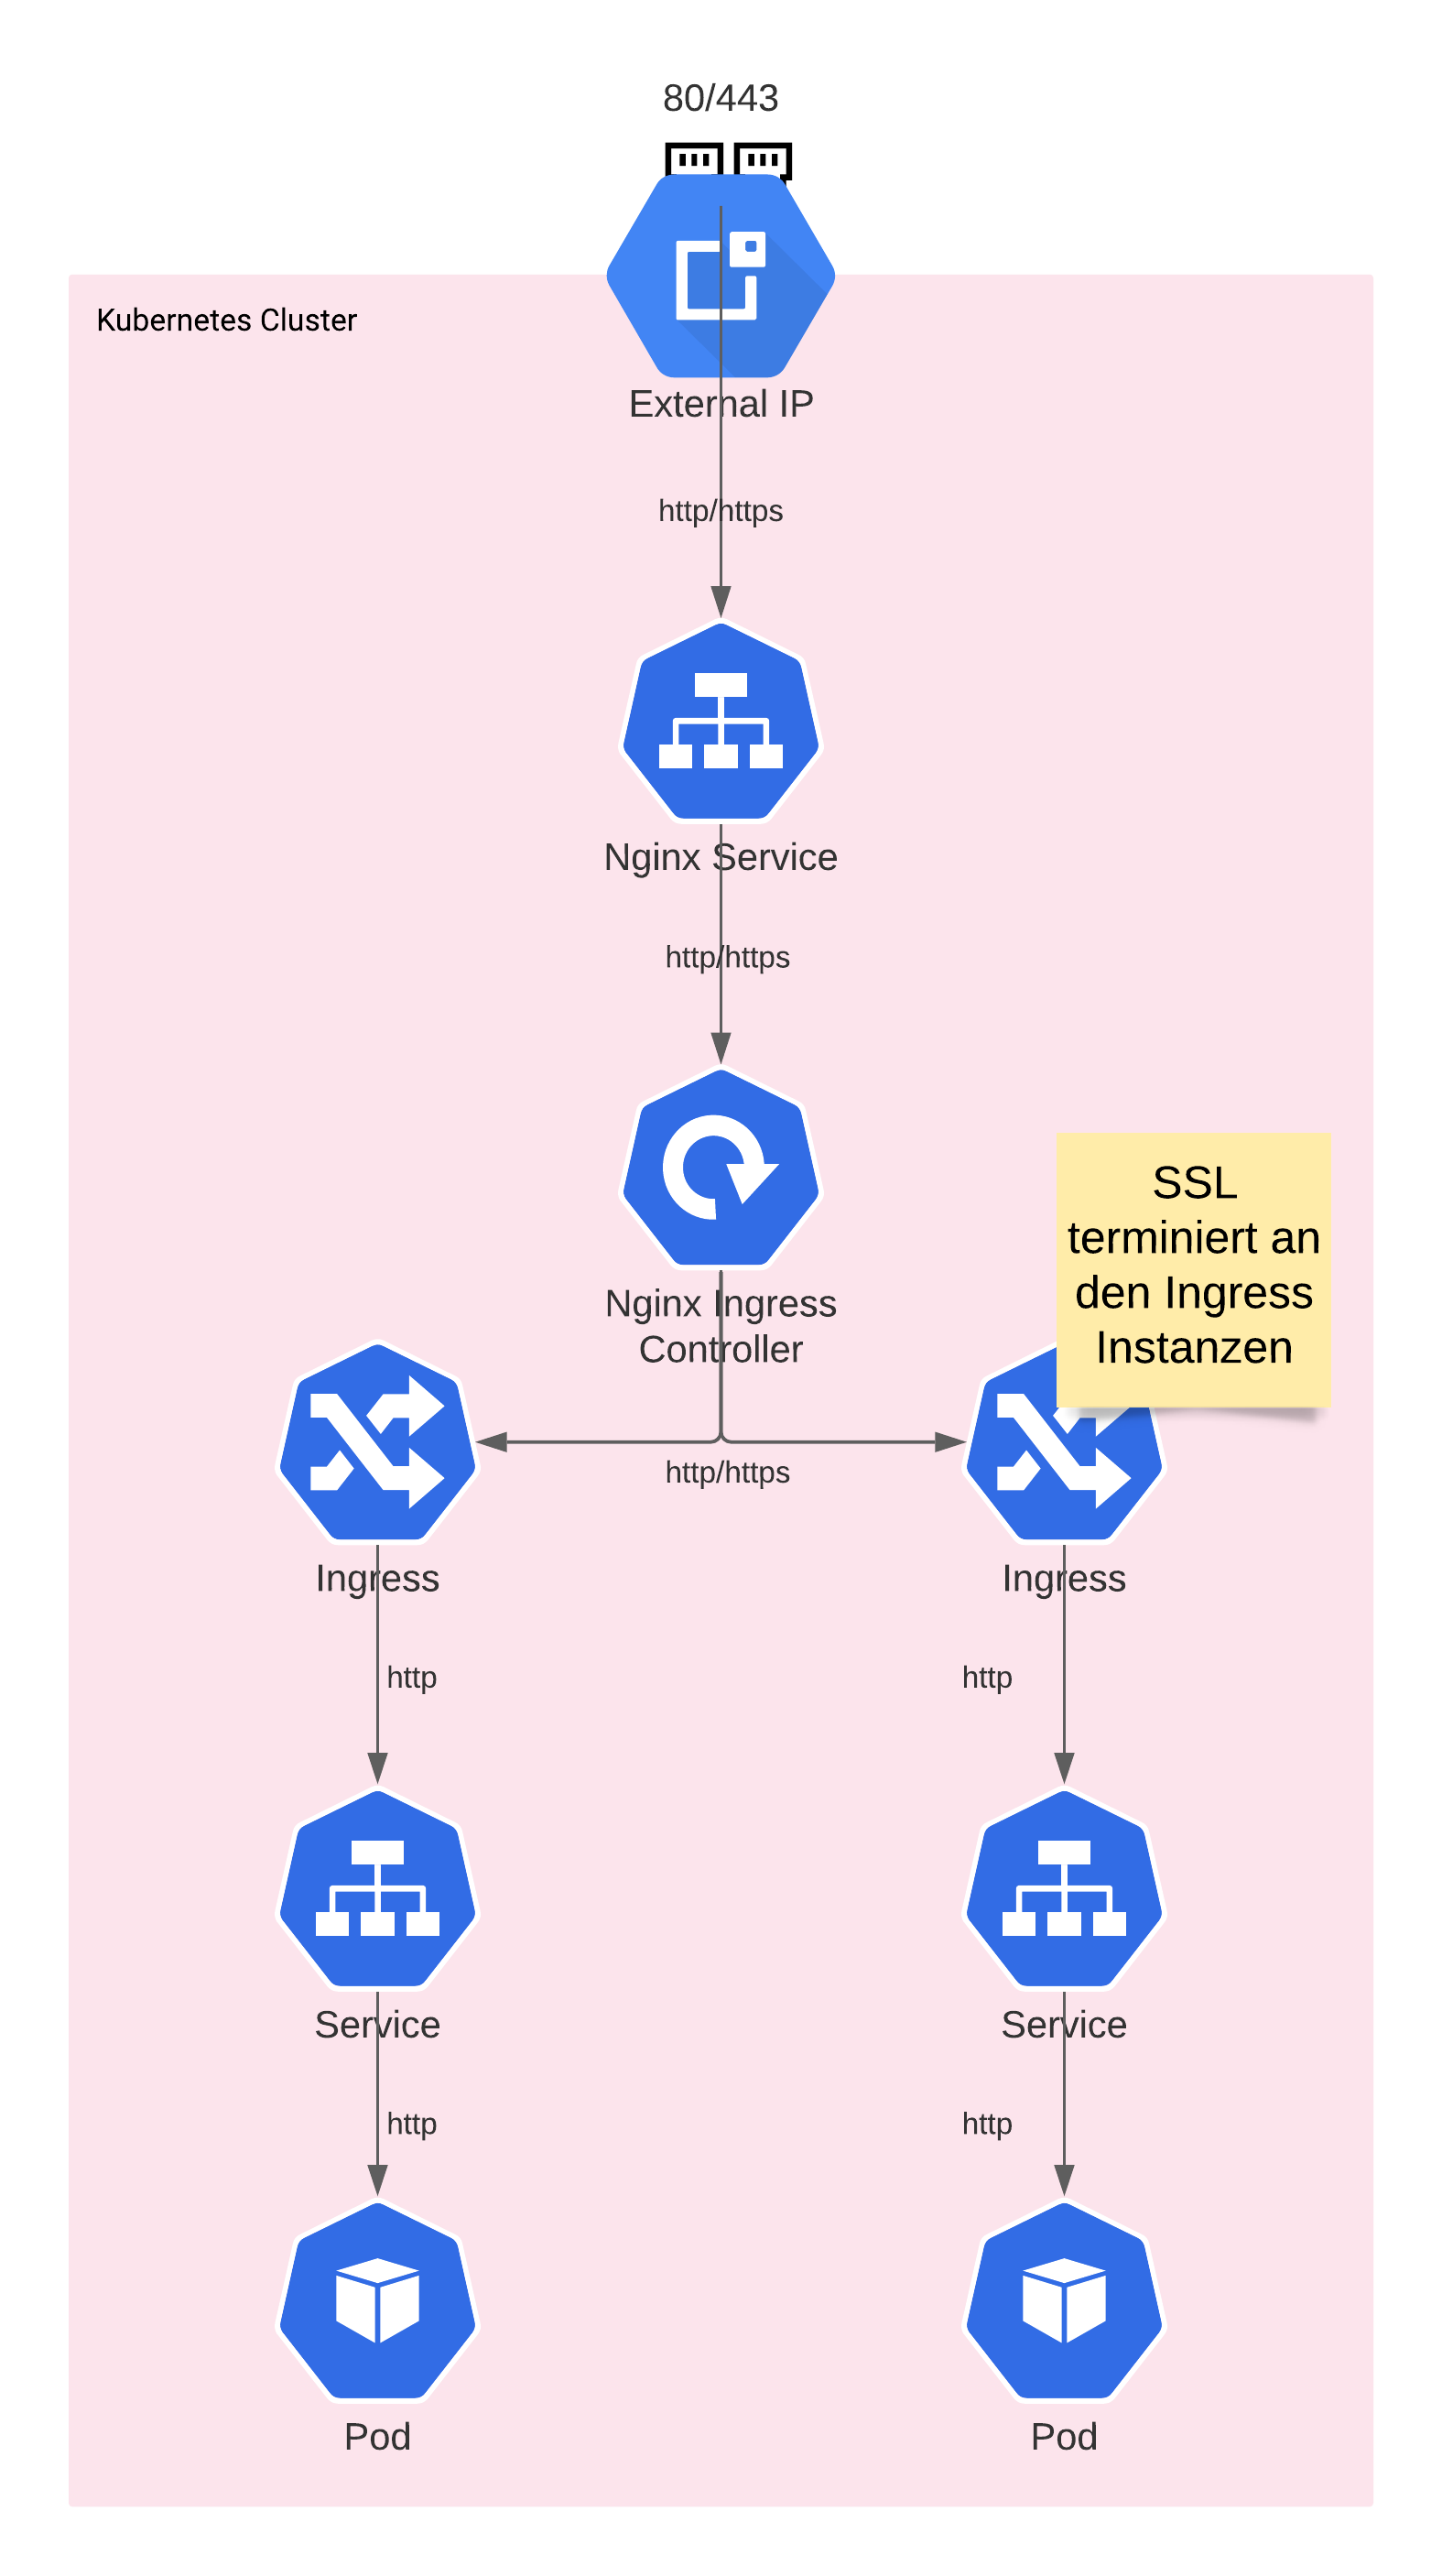
\includegraphics[width=0.8\textwidth]{bilder/ClusterIP.png}
    \caption{Ingress Cluster IP Architektur}
    \label{fig:clusterip}
\end{figure}
Zum Deployment des Ingress wurde die Standart-Anleitung\footnote{https://github.com/nginxinc/kubernetes-ingress} verwendet.
Die einzige Änderung ist hier das Umändern des Service Typen zu einer externalIP und das Freigeben der entsprechenden Ports.
Diese Änderungen sind dem Anhang unter \ref{app:clusterip} beigefügt.
\\
Das Deployment wird über Ansible gemanaged, in dem Playbook werden die nötigen \ac{YAML} Konfigurations Dateine auf den Master kopiert und dann mittels \textbf{kubctl apply} angewandt. 


\subsubsection{Storage}
Um mit \ac{PV}s arbeiten zu können muss dafür ein Provider vorhanden sein, der den angefragten Block Storage zur Verfügung stellen kann. 
In den Cloud Umgebungen wird das, wie auch die Load Balancer, von dem Cloud Provider gemanaged. 
Auf der bare metal Lösung muss dies eigenständig getan werden, mit Software-Lösungen wie Longhorn.\footnote{https://longhorn.io}
Longhorn erstellt für jedes Volume einen dedizierten Storagfe Controller und repliziert das Volume über verschiedene Nodes.
Damit wird die Persistenz gewährleistet.
Durch ein DaemonSet wird auf jedem Node ein Manager Pod gehostet, der für das erstellen und managen von den Volumes der Nodes zuständig ist. 
\\
Longhorn wird über \textbf{helm} installiert. 
Um Helm zu installieren wird zunächst die Installationsanleitung\footnote{https://helm.sh/docs/intro/install/} in Ansible abgebildet.
Diese beinhaltet das Hinzufügen der Verschlüsselungs Keys und des helm-Repositorys zu \textbf{apt}, das Installieren des \textbf{apt-transport-https} Pakets, und schließlich das Installieren des Helm Pakets.
\\
Wenn das Helm Paket installiert ist wird das Longhorn Repository über das \textbf{git} Modul hinzugefügt, ein Namespace für longhorn angelegt und dann Longhorn deloyed.
Die komplette Rolle ist dem Anhang unter \ref{app:longhorn} beigefügt.

\subsubsection{Dashboard}
Die letzte Funktionalität, die für ein vollwertiges Kubernetes-Cluster noch fehlt, ist eine Möglichkeit, die Pods in irgendeiner weise zu monitoren.
Das Kubernetes Dashboard bietet simple Monitoring-Funktionen sowie die Möglichkeit Änderungen durchzuführen, Ressourcen zu löschen, erstellen und einzusehen.
Um das Dashboard zu installieren wurde mit der aktuellen Installationsanleitung\footnote{https://kubernetes.io/docs/tasks/access-application-cluster/web-ui-dashboard/} von Kubernetes gearbeitet.
Zum Zugriff auf das Dashbaord muss User und ein ClusterRoleBinding erstellt werden. 
Mit dem Token dieses Users kann sich dann an dem Dashboard angemeldet werden, um dieses sinnvoll nutzen zu können.\footnote{https://github.com/kubernetes/dashboard/blob/master/docs/user/access-control/creating-sample-user.md}

\todo{monospaceschriftart}

	\chapter{Migration von Sormas}

\section{SORMAS}
\label{ref:sormas_strucure}
Um die Anwendung \ac{SORMAS-ÖGD}(im weiteren zur Vereinfachung nur noch \ac{SORMAS}) erfolgreich migrieren zu können, müssen wir diese in ihre einzelnen Teile aufteilen und identifizieren wofür die einzelnen Komponenten verantwortlich sind.
Da \ac{SORMAS} zum aktuellen Zeitpunkt als containerisierte Anwendung ausgerollt wird, kann die \textit{docker-compose.yaml}\footnote{https://github.com/hzi-braunschweig/SORMAS-Docker/blob/master/docker-compose.yml} des Projekts als Orientierung genutzt werden.
Diese beschriebt 5 Container, die zusammen die Anwendung bilden.
\begin{itemize}
    \item sormas-application \\ Der Payara-Server auf dem die \ac{SORMAS}-Applikation gehostet wird.
    \item sormas-postgres \\ Die Datenbank in der die Daten aus der Anwendung gespeichert werden.
    \item sormas-pg-dump \\ Dieser Container ist ausschließlich dafür verantwortlich in bestimmten Zeitabständen einen Datenbank Dump der Postgres-Datenbank zu machen.
    \item sormas-apache2 \\ Der Webserver ist für die Terminierung der \ac{SSL}-Zertifikate verantwortlich
    \item autoheal \\ Damit können gestoppte oder ungesunde Container neu gestartet werden
\end{itemize}
Da die Anwendung nach Kubernetes migriert werden soll, können einige der Funktionen von den Kubernetes-eigenen Funktionalitäten übernommen werden. 
Der Ingress kann die Terminierung der \ac{SSL} Zertifikate managen und wird den Apache Webserver ersetzen.
Die Autoheal-Funktion gehört zu den Grundfunktionen von Kubernetes und muss nicht extra implementiert werden, wenn die Anwendung als ReplicaSet oder Deployment ausgerollt wird.
Der Container, der nur die Datenbank Dumps ausführt, kann durch einen Cronjob abgebildet werden. 
Die einzigen Container die dann noch übernommen werden sind der Payara-Server und die PostgreSQL-Datenbank.
Zusätzlich müssen Ingress und Cronjob konfiguriert werden. \\
Doch zunächst sollen einzelne Funktionen von Kata getestet werden.


\section{Erste Tests mit der Kata Runtime}
\label{ref:lokale_kata_tests}
Noch bevor begonnen wurde das Cluster aufzubauen, wurden erste Test mit der Kata-Runtime durchgeführt. 
Mit diesen wurde überprüft ob schon im voraus Probleme identifiziert werden konnten, die die Umsetzung verhindern würden. 

\subsection{Docker Kata Integration}
Als erstes wurde ein Container in der Kata Runtime über die bereits installierte Container Engine Docker gestartet.
Mit dem Command \texttt{uname -a} kann der in dem Container verwendete Kernel ausgegeben werden. 
Wenn dieser mit dem Kernel des Host Systems verglichen wird, kann festgestellt werden ob beide auf dem gleich Kernel laufen, wie es bei Docker Containern der Fall wäre, oder ob ein eigener Kernel für die VM virtualisiert wurde.
\\
Über Docker lassen sich Kata-Container mit dem Parameter \texttt{--runtime=kata} starten.
Als Images wurden kleine Alpine-Container gewählt.
Um einen Vergleich zwischen beiden Runtimes ziehen zu können wurde ein kurzen Skript geschrieben, dass die StartUp-Zeiten in eine Datei schreibt.
Das Skript unter \ref{lst:startuptimes} ergab auf meiner Maschine eine zeitliche Differenz von ca. einer Sekunde wie aus \ref{app:startuptimecomparison} zu entnehmen ist. 
Die wichtigste Erkenntnis an dieser Stelle ist jedoch, dass die Container in der neuen Runtime problemlos starten, und dazu tatsächlich einen anderen Kernel gestartet bekommen.

\begin{lstlisting}[language=bash, caption={compare\_startup\_times.sh}, label=lst:startuptimes]
#!/bin/bash
touch startuptime_comparison
echo runc: > startuptime_comparison
{ time docker run --rm --runtime=runc archlinux sh -c 'uname -r'; } 2>> startuptime_comparison
echo kata-runtime: >> startuptime_comparison
{ time docker run --rm --runtime=kata archlinux sh -c 'uname -r'; } 2>> startuptime_comparison
\end{lstlisting}

\subsection{Webapp in Kata}
\label{ref:kata_plug_and_play}
Im nächsten Test soll das Deployment einer Web-Anwendung in Kata gestestet werden. 
Dafür wurde das Docker-Image einer Website zum Thema der Web\ac{API}s, das während des letzten Semesters erstellt wurde, gewählt\footnote{https://hub.docker.com/r/robbmue/webapi}. 
Tatsächlich mussten hier gar keine Anpassungen vorgenommen werden. 
Der \texttt{runtime}-Parameter wurde gesetzt und beim Start konnte der andere Kernel nachgewiesen werden.
Ansonsten werden keine Änderungen in dem Verhalten der Anwendung festgestellt. 
Das Austauschen der Runtime verlief vollständig nach dem von Kata angestrebten Plug-and-Play Prinzip.
Hier wurden die Möglichkeiten, die durch das einheitliche Verwenden der Schnittstellen ermöglicht werden, deutlich. 

\subsection{PostgreSQl in Kata}
\label{ref:postgres_kata}
Als letzter grundlegender Test sollte eine PostgreSQL Anwendung in der Kata-Runtime deployed werden. 
Während sich zuvor die Runtime ohne Änderungen an dem Verhalten der Applikation austauschen ließ, konnten hier zum ersten Mal Unterschiede registriert werden.
\\
Das Starten der Anwendung war noch sehr unproblematisch, alle benötigten Variablen konnten über eine enviroment-Datei übertragen werden und die Runtime wie zuvor über den entsprechenden Parameter definiert werden. 
Wurde der Container nach dem Start der Anwendung jedoch betreten und man versucht von dort aus in die Postgres Datenbank zu kommen, erhielt man folgenden Fehler:
\\\texttt{could not connect to server, temporary failure in name resolution}\\
Die Datenbank ist allerdings von außerhalb erreichbar.
Wurde kein \texttt{docker exec} in den Container ausgeführt, sondern direkt von der Host-Maschine aus der Zugriff auf die Datenbank gestartet, konnte diese ohne Probleme bedient und gemanaged werden. 
Das Problem ließ sich zwar in der dafür eingeplanten Zeit nicht lösen, da die Datenbank aber trotzdem erreicht wurden konnte, sollte diese Einschränkung keine Behinderung darstellen. 

Die grundlegenden Tests können damit als abgeschlossen betrachtet werden und es kann mit dem nächsten Schritt, dem Übersetzen der \textit{docker-compose.yaml} zu Kubernetes Manifesten, begonnen werden. 
Zunächst muss dieser Schritt getan werden, damit anschließend die Runtime auf Kata umgestellt und dann gedebugged werden kann. 


\section{Migration der Anwendung nach Kubernetes}
\subsection{Struktur}
Als erstes wurde die Struktur der Kubernetes Anwendung geplant. 
Wie schon in Absatz \ref{ref:sormas_strucure} festgehalten, können einige Container ignoriert werden, da Ihre Funktion standartmäßig in Kubernetes integriert ist. 
Die restlichen Container müssen jedoch zu Deployments oder StatefulSets übersetzt, mit Services zugänglich gemacht, und mit Secrets sowie ConfigMaps konfiguriert werden. 
Außerdem müssen den Anwendungen \ac{PV}s zugeordnet werden und sie müssen mittels eines Ingress erreichbar gemacht werden.
Der genaue Aufbau wurde in Abbildung \ref{fig:sormas_kubernetes} dargestellt. 
Aus Gründen der Übersichtlichkeit wurde hierbei auf die Darstellung der Backup-Funktionalitäten verzichtet, diese werden später genauer erklärt.

\begin{figure}[h!]
\centering    
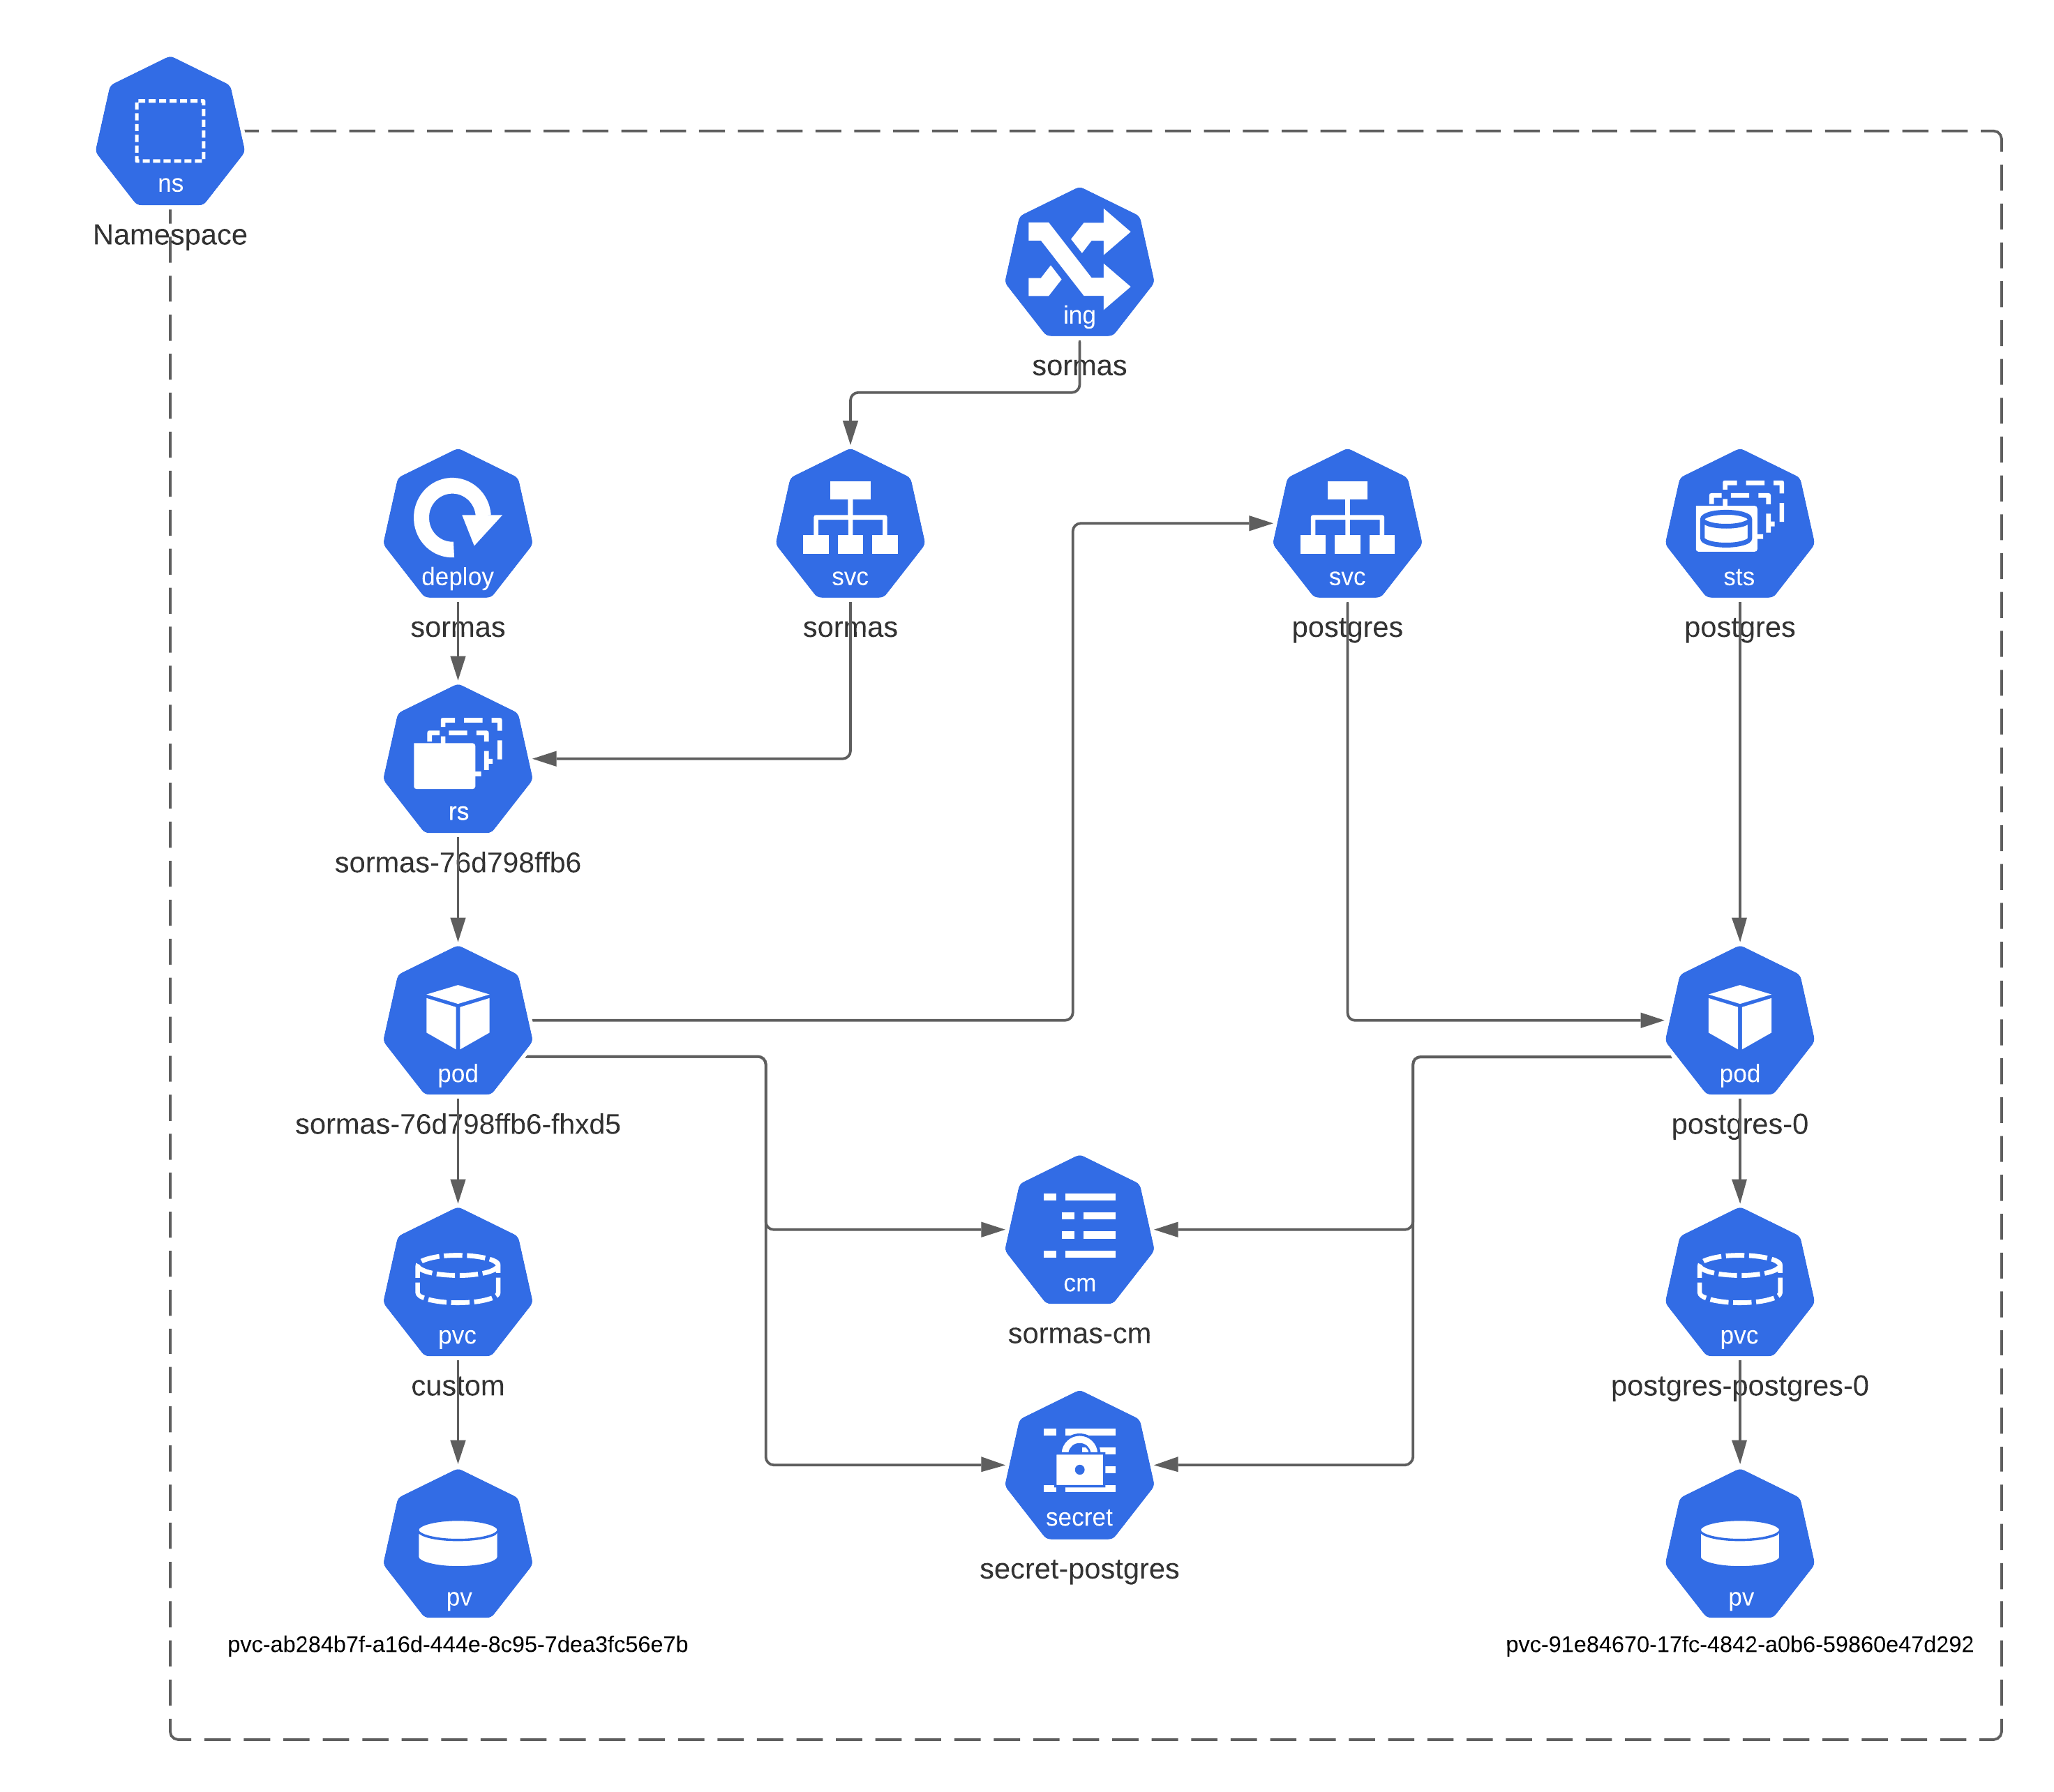
\includegraphics[width=\textwidth]{bilder/sormas_kubernetes.png}
\caption{SORMAS in Kubernetes}
\label{fig:sormas_kubernetes}
\end{figure}

Als Element zur Trennung und Organisation der einzelnen \ac{SORMAS}-Instanzen wird für jedes \ac{GA} ein eigener Namespace angelegt.
So kann jeder Pod genau einem \ac{GA} zugeordnet werden.\\
Wie zuvor angemerkt, ersetzt der Ingress an dieser Stelle den zuvor zur \ac{SSL}-Terminierung benötigten Apache2 Webserver.\\
Eine Datenbank wird in einem StatefulSet ausgerollt, da diese durch die genaue Bestimmung der Pods besser persistent gestaltet werden kann.
Ein StatefulSet erstellt dann seinen benötigten Pod, der über ein \ac{PVC} sein \ac{PV} zugeordnet bekommt. 
Die Konfiguration des Pods soll ausschließlich in der ConfigMap und dem Secret stattfinden, sodass nur an einer Stelle Anpassungen vorgenommen werden müssen.
Der Pod kann durch das Einrichtigen eines Services für andere Instanzen im selben Namespace erreichbar gemacht werden.\\
Der Payara-Server wird mit einem Deployment-Manifest ausgerollt. 
Eigenschaften des StatefulSets werden nicht benötigt und Vorteile in Hinsicht auf das erleichterte Updaten der Software werden für zu erwartende Updates nützlich sein.
Das Deployment erstellt dann das entsprechende ReplicaSet und dieses den Pod. 
\ac{PV} und Konfiguration werden analog zu Postgres gemanagt. 
Der Service wählt mittels des Selectors allerdings das ReplicaSet und nicht den Pod selbst.


\subsection{Schreiben der Kubernetes Manifeste}

Alle geschriebenen Manifeste, auch die auf die in diesem Abschnitt nicht weiter eingegangen wird, sind auf Github veröffentlicht und können dort unter \url{https://github.com/robbmue/katanetes_sormas/tree/master/manifests} eingesehen werden. 

Beim Schreiben der Manifeste diente die \textit{docker-compose.yml}\footnote{https://github.com/hzi-braunschweig/SORMAS-Docker/blob/master/docker-compose.yml} als Vorlage.
Aus dieser wurden zunächst einmal alle Services eliminiert die in Kubernetes nicht weiter benötigt werden, namentlich der Autoheal, der Apache2 Webserver und der pg-dump.
Die beiden letzten Teile der Anwendung wurden dann entsprechend der vorhergehenden Planung in jeweils ein Deployment und ein StatefulSet übersetzt.
Zuerst wurde ein Namespace für die komplette Anwendung angelegt, in dem alle restlichen Teile deployed werden.

\hfill \newline
\subsubsection{Payara Deployment}
Bei dem Payara Server ist vor allem wichtig, deren speziellen Port in das Manifest miteinzubinden.
Payara nutzt als Standart-Port 6080 und als Admin-Port 6048, diese werden unter den Namen \texttt{payara} und \texttt{payara-admin} dem Deployment hinzugefügt.
Abhängig von diesen ist auch die liveness- und readinessProbe, hier werden diese mit einem \ac{HTTP}-GET auf den entsprechenden Port und den \ac{SORMAS}-Pfad \texttt{/sormas-ui/login} realisiert.
Wenn diese Seite erreichbar ist, kann von einer funktionierenden Instanz ausgegangen werden.
Der Service, der auf diese Anwendung verweist, wird so konfiguriert, dass dieser auf Port 80 lauscht aber alle eingehenden Anfragen an Port 6080 des Payara-Pods weiterleitet.
So kann der ungewöhnliche Port des Payara-Servers in einen Standart-Port umgewandelt werden. 
Der Ingress wiederum zeigt auf den Service und Sorgt dafür, dass die Anwendung von außerhalb erreichbar ist.

Des weiteren muss das \ac{PV} mittels des \ac{PVC} eingebunden werden und die Enviroment-Variablen müssen gesetzt werden. 
Der \ac{PVC} wird unter dem Punkt \texttt{volumes} dem Pod zugewiesen und unter \texttt{volumeMounts} wird der Pfad angegeben, an der das Volume eingehängt werden soll. 
Die Variablen setzt man unter dem Punkt \texttt{env}, hier kann sowohl auf ein Secret, als auch auf eine ConfigMap zugegriffen werden.
Es könnten auch direkt in dem Deployment die korrekten Werte gesetzt werden, mit der ConfigMap und dem Secret wird jedoch erreicht, dass Änderungen nur an möglichst wenigen Stellen vorgenommen werden müssen.
Außerdem wird auch das StatefulSet auf die gleichen Dateien zugreifen, und so kann garantiert werden, dass beide Anwendungen übereinstimmende Werte geliefert bekommen.

Zuletzt werden noch Limits für \ac{CPU} und Memory-Nutzung gesetzt. 

Auf die Manifeste für den \ac{PVC}, die ConfigMap und das Secret soll hier nicht weiter eingegangen werden. 

\subsubsection{SORMAS StatefulSet}
Für die Datenbank wurden Konfigurationen analog zu denen des Payara-Servers vorgenommen.
Der Port 5432 wurde freigegeben, die Enviroment Variablen und der \ac{PVC} wurden eingebunden sowie Limits gesetzt.
Eine Besonderheit in diesem Manifest ist, dass mit dem \texttt{args} Parameter gearbeitet werden muss. 
Es muss eine Änderung an dem Parameter \texttt{max\_prepared\_connections} in der \textit{postgresql.conf} vorgenommen werden, damit \ac{SORMAS} starten kann. 
Der Postgres Container startet immer mit dem \texttt{psql} Kommando, also kann mittels des Arguments \newline
\texttt{-c config\_file=/etc/postgresql/postgresql.conf} die Config eingelesen werden.

Auf den Service und den \ac{PVC} soll an dieser Stelle nicht weiter eingegangen werden, sie können auf Github nachgelesen werden. 


\subsubsection{Backup}
Als Backup-Lösung wurde Stash\footnote{https://stash.run/\#} von AppsCode\footnote{https://appscode.com/} gewählt.
Die Software erlaubt es unter anderem Backups auf einem lokalen Storage zu erstellen und mit Datenbank Dumps zu arbeiten, nicht nur mit Volume Snapshots.

Bei Netzlink wird ein lokaler Minio\footnote{https://min.io/} \ac{S3}-Storage gehostet, in dem die Backups gespeichert werden können.
Damit Stash die Verbindung zu diesem aufbauen kann muss zunächst ein Secret erstellt werden, dass die Anmeldedaten für den \ac{S3} Storage beinhaltet.
Aufbauend darauf kann dann die \ac{CRD} \texttt{Repository} deployed werden. 
Diese gibt die Adresse des \ac{S3} Storage an, sowie den Bucket in den gespeichert werden soll und das zur Organisation verwendete Prefix.
Außerdem beinhaltet die Repository-Ressource auch das zuvor definierte Secret und bindet dieses so an das Repository.
\\
Als nächstes wird die \ac{CRD} \texttt{AppBinding} erstellt. 
Dieses AppBinding wird benötigt um auf die Datenbank zuzugreifen. 
Dazu braucht es den Service und Port, sowie das Schema und den Typen der Datenbank und letzten endes ein Secret, aus dem der Datenbanknutzer und sein Password ausgelesen werden können.
In dieser einen \ac{CRD} sind dann also alle Informationen gesammelt um auf die Datenbank zuzugreifen und in dem Repository ist definiert wohin das Backup gespeichert werden soll.
Als letztes fehlt also nur noch eine Ressource, die das Backup anstößt.
\\
Diese \ac{CRD} nennt sich \texttt{BackupConfiguration}. 
In ihr wird 
\begin{itemize}
    \item das \texttt{AppBinding} und das \texttt{Repository} zusammengetragen
    \item der auszuführende Task angegeben (in dem Version und Art der Datenbank festgelegt sind)
    \item eine \texttt{retentionPolicy} definiert (diese gibt an wie viele der erstellten Backups erhalten bleiben sollen)
    \item der \texttt{schedule} in CronJob Syntax angegeben
\end{itemize}
Stash erzeugt aus diesen \ac{CRD}s dann Ressourcen, mit denen Kubernetes arbeiten kann.
Alle benötigten Informationen werden in einem Kubernetes nativen CronJob zusammengetragen.
Ein CronJob in Kubernetes erstellt immer zur definierten Zeit eine Job-Ressource. 
Ein Job wiederum erstellt einen oder mehrere Container, die nur eine genau abgegrenzte Aufgabe haben, und stellt sicher dass diese erfolgreich terminieren. 
In diesem Fall ist die Aufgabe das Erstellen das Datenbank Dumps, das Verschlüsseln und Kopieren der verschlüsselten Daten auf den \ac{S3} Storage plus das Löschen der überschüssigen, bereits vorhandenen Datenbank Dumps.
Nach der erfolgreichen Ausführung all dieser Operationen terminiert der Job und alle Pods werden gestoppt. 
So kann garantiert werden, dass das Backup nur während der Ausführung Compute-Ressourcen verbraucht. 

Wird nun eine \ac{SORMAS}-Instanz mit diesen Manifesten deployed ist die komplette Funktionalität der ursprünglichen Anwendung abgebildet.

\subsubsection{Tests}
\label{ref:tests}
Als erstes wurde kontrolliert, ob der Payara Server erreichbar ist.
Dazu muss ein Host-Eintrag auf dem Localhost gesetzt werden, da das Test Cluster nicht in der \ac{DMZ} aufgebaut wurde, keinen \ac{DNS} Eintrag hat und nur aus dem Netzlink-Netzwerk zu erreichen ist. 
Wenn der Payara-Server erreichbar ist, wird als nächstes überprüft, ob das \ac{SORMAS}-\ac{GUI} erreichbar ist.
Auf der \ac{GUI} kann dann gecheckt werden, ob mit dem konfigurierten Usern eine Anmeldung durchgeführt werden kann und somit der Login Prozess funktioniert.
Nachdem die Anmeldung durchgeführt wurde, werden einige Fälle eingetragen, bearbeitet und gelöscht um die Funktionalität der Anwendung sowie die Postgres Integration zu prüfen.

Um die Autoheal-Funktion zu testen, kann einfach der Sormas Pod gelöscht und dann die Erstellung des neuen Pods abbgewartet werden.
Wenn dieser von dem ReplicaSet wieder gebaut wird, ist die Autoheal-Funktion korrekt abgebildet.

Zuletzt wird die BackUp-Funktion überprüft.
Dazu werden einige Einträge in der Datenbank vorgenommen, und ein BackUp-Job angestoßen. 
Nachdem dieser durchgelaufen ist werden die Daten aus der PostgreSQL-Datenbank gelöscht.
Über einen Restore-Job wird versucht die zuvor gelöschten Daten aus dem Datenbank Dump wiederherzustellen. 
Wenn der Restore-Job erfolgreich beendet wird und die Daten wieder in der Anwendung auftauchen, ist die Backupfunktionalität positiv getestet.


\section{Migration der Anwendung zur Kata-Runtime}
Theoretisch funktioniert die Migration der Anwendung nach dem gleichen Plug-and-Play Prinzip wie bereits in Abschnitt \ref{ref:kata_plug_and_play} beschrieben.
Die Runtime ist für Containerd bereits in Abschnitt \ref{ref:kata_config} als Plugin definiert und muss nur als Parameter in die Manifeste eingepflegt werden.
Der Parameter wird wie im Quelltext \ref{lst:runtimeClassName} gesetzt.
Leider ließ sich dieses Verfahren jedoch in der Praxis nicht so problemlos umsetzen, die Probleme und Lösungen sollen in den nächsten Absätzen aufgezeigt werden. 

\begin{lstlisting}[language=yaml, caption=runtimeClassName, label=lst:runtimeClassName]
apiVersion: apps/v1
kind: Deployment
metadata:
  name: sormas
  namespace: ga-test
spec: 
  replicas: 1
  selector: 
    matchLabels:
      run: sormas
  template:
    metadata:
      labels:
        run: sormas
    spec:
      runtimeClassName: kata
      containers:
        - image: hzibraunschweig/sormas-application
          name: sormas
...
\end{lstlisting}


\subsection{Migration des Payara Servers}
\label{ref:payara_kata}
Der Payara Server wurde als erstes zur Migration ausgewählt. 
Der Parameter wurde entsprechend gesetzt und die komplette Anwendung wurde ausgerollt. 

Zuerst schien es als würde die Anwendung auf dem Payara-Server gar nicht starten. 
Der Payara Server selbst war zwar erreichbar, doch die Anwendung darauf war nicht erreichbar.
Beim genaueren Beobachten des Server wurde festgestellt, dass die \ac{SORMAS}-\ac{GUI} für einige Sekunden erreichbar ist und sogar die Anmeldung durchgeführt werden kann, bis die \ac{GUI} aus irgendeinem Grund wieder verschwandt.
In den Logs wurden tausende Zeilen Java Stack Traces ausgegeben.
Die Analyse der Logs ergab, dass die Anwendung zu einem bestimmten Zeitpunkt \texttt{successfully autodeployed} wurde, der Payara-Server aber nicht wie unter runc an dieser Stelle den Deployment Process beendete sondern wieder damit begann die Anwendung zu deployen.
Als diese Erkenntnis gewonnen war, wurde untersucht welche Dateien zu welchem Zeitpunkten im Filesystem erstellt wurden und wie sich diese von dem Deployment-Prozess in runc unterscheiden. 
Es war jedoch keine Abweichung während des Deployments festzustellen.
Auch nach langer intensiver Recherche und Troubleshooting mit qualifizierten Kollegen konnte kein Grund dafür gefunden werden, dass das Autodeployment nicht nach dem erfolgreichen Ausrollen der Anwendung stoppt. 
\\
Das Autodeployment Feature von Payara muss also für unseren Use-Case umgangen werden. 
Dazu wurden die offiziellen Dockerfiles der \ac{SORMAS}-Applikation\footnote{https://github.com/hzi-braunschweig/SORMAS-Docker/tree/master/sormas} untersucht. 
In diesem werden die Skripte \textit{setup-server.sh} und \textit{start-server.sh} genutzt.
In dem \textit{start-server.sh} Skript zum Deployen der Anwendung werden als letztes alle \textit{.ear} und \textit{.war} Dateien in den Autodeployment-Ordner kopiert.
Wird dann der Payara-Server mittels \texttt{asadmin start-domain} gestartet versucht der Server alle Dateien in dem Autodeployment-Ordner auszurollen.
Um zu verhindern, dass der Autodeployment-Prozess die Anwendung immer wieder zerschießt, muss Sie auf einem anderen Weg ausgerollt werden.
Dazu wurde das \textit{start-server.sh} Skript entsprechend angepasst, sodass die einzelnen \textit{.ear} und \textit{.war} Dateien mittels des \texttt{asadmin deploy} Kommandos ausgerollt werden.
Mit diesen Änderungen wird die Autodeployment-Funktion komplett ausgesetzt, sodass die Anwendung nun nicht mehr vom Payara-Server selbst zerstört werden sollte.
Es wurde ein neues Container-Image mit diesen Anpassungen erstellt und auf der Docker-Registry\footnote{https://hub.docker.com/repository/docker/robbmue/sormas\_kata} veröffentlicht, damit Kubernetes dieses Image herunterladen kann.
Nachdem das neue Image in die Manifeste eingebunden, und die Anwendung neu ausgerollt wurde, konnte mit den zuvor unter Abschnitt \ref{ref:tests} beschrieben Tests gezeigt werden, dass der \ac{SORMAS}-Payara nun unter Kata voll funktionsfähig war.


\subsection{Migration der PostgreSQl-Datenbank}
\ref{ref:postgres_kata}
Als nächster und letzter Teil der Anwendung muss nun noch die Datenbank mit ihrem eigenen Kernel versehen werden.
Dazu wurde zuerst wieder der benötigte Parameter in dem StatefulSet Manifest gesetzt und anschließend die Anwendung ausgerollt.

Nach ausführlichen Tests mit dem Image des \ac{HZI} konnte jedoch keine Kommunikation zwischen der Java-Applikation und der Datenbank aufrecht erhalten werden.
Um die Probleme zu verstehen wurde mit allen möglichen Postgres-Images experimentiert.
Nach einigen weiteren Tests stand fest, dass die Probleme ausschließlich in den Alpine-Versionen der Postgres Images auftreten, aber nicht in den Postgres Images auf Debian Basis. 
Die Herausforderung besteht also darin, das Image des \ac{HZI}, das auf dem Postgres-Image auf Alpine Basis aufbaut, in einem neuen Image abzubilden, das auf dem Postgres-Debian Image basiert.
Die Alpine Version wurde vermutlich gewählt um den Container möglichst klein zu halten. 
In \ref{lst:alpine_postgres_size} wird die Größe des Images ermittelt.
Diese beträgt \texttt{450MB}.

\begin{lstlisting}[language=bash, caption={Größe des ursprünglichen Postgres Images}, label=lst:alpine_postgres_size]
$  ~ docker images | awk 'NR==1 || /^hzibraunschweig\/sormas-postgres/ {printf "%-33s %-10s %s\n", $1, $2, $NF}'
REPOSITORY                        TAG        SIZE
hzibraunschweig/sormas-postgres   2.8.0      450MB
\end{lstlisting}

Die Untersuchung des Images ergab, dass sehr viele Pakete installiert werden müssen um das Modul \texttt{temporal\_tables} für Postgres zu installieren.
Die folgenden Pakete werden benötigt um das Modul zu installieren und zu compilieren:
\begin{itemize}
  \item postgresql-server-dev-10
  \item pgxnclient 
  \item make
  \item gcc
\end{itemize}

Nach der Installation des Moduls werden sie jedoch nicht mehr benötigt und können deswegen mittel des \texttt{apt}-Feature \texttt{autoremove} wieder entfernt werden. 
So wird versucht das Image trotz der größeren Basis klein zu halten.
Eine Überprüfung der Image-Größe nach dem Bauen ergab, dass das Image durch die Anpassungen sogar kleiner geworden ist und nun nur noch \texttt{373MB} beträgt, wie \ref{lst:debian_postgres_size} zeigt.

\begin{lstlisting}[language=bash, caption={Größe des Debian Images}, label=lst:debian_postgres_size]
$  ~ docker images | awk 'NR==1 || /^robbmue\/postgres_kata/ {printf "%-33s %-10s %s\n", $1, $2, $NF}'
REPOSITORY                        TAG        SIZE
robbmue/postgres_kata             latest     373MB
\end{lstlisting}

Es wurde ein neues Container-Image mit diesen Anpassungen erstellt und auf der Docker-Registry\footnote{https://hub.docker.com/repository/docker/robbmue/postgres\_kata} veröffentlicht, damit Kubernetes dieses Image pullen kann.
Nachdem das neue Image in die Manifeste eingebunden, und die Anwendung neu ausgerollt wurde, konnte mit den zuvor unter Abschnitt \ref{ref:tests} beschrieben Tests gezeigt werden, dass die Postgres-Datenbank nun unter Kata voll funktionsfähig ist.

Das neue Postgres-Dockerfile ist dem Anhang unter \ref{app:small_postgres} zu entnehmen.


\section{Helm Templating}
Im letzten Schritt soll das Deployment nun soweit vereinfacht werden, dass das Bereitstellen einer kompletten Instanz über einen einzigen Befehl durchgeführt werden kann.
Dazu wird \texttt{helm} eingesetzt. 
Die Software bietet vielfältige Möglichkeiten, von denen für dieses Projekt jedoch nur die Templating-Funktion genutzt wird.
Für jedes \ac{GA} soll ein eigener Namespace erstellt werden, zuerst wird also die Namespace Ressource getemplatet.
Für den Namespace wird der Release-Name verwendet, sodass dafür nichtmal die \textit{values.yaml} angepasst werden muss, in der alle anderen Variablen für das Templating gesetzt werden. 
Der Release-Name wird direkt in dem \texttt{helm install} Befehl mit angegeben, die Syntax ist unter \ref{lst:helm_install} beschrieben, in dem Beispiel wäre das "beispielgesundheitsamt".
Im Anhang unter \ref{app:namespace_template} wird gezeigt wie mit dem Release Name gearbeitet wird. 
Analog dazu werden die Namespaces aller anderen Ressourcen definiert. 

\begin{lstlisting}[language=bash, caption={Syntax des \texttt{helm install} Kommanods}, label=lst:helm_install]
helm install <beispielgesundheitsamt> ./sormas
\end{lstlisting}

Alle anderen Variablen werden über die \textit{values.yaml} gesetzt.
In dieser kann mit Objekten gearbeitet werden, für dieses Projekt gibt es beispielsweise ein Objekt \texttt{image} das die Objekte \texttt{sormas} und \texttt{postgres} enthält, in denen dann Name und Version des Images definiert wird. 
Dieses Beispiel ist dem Anhang unter \ref{app:values_yaml} beigefügt.
Auf diese Werte wird ähnlich wie auf den Release-Name zugegriffen, nur dass der Release durch Values ersetzt wird.
Auf den Sormas Image Namen mit Version wird folgenderweise zugegriffen: \texttt{ \{\{ .Values.image.sormas.name \}\}:\{\{ .Values.image.sormas.version\}\} }

Helm bietet auch die Option, Werte die aus der Values-Datei eingelesen werden in Pipelines zu senden um sie in beliebiger Art zu transformieren. 
Diese Funktionalität ermöglicht es, die Werte für die Secrets im Klartext in die Values zu schreiben, um sie dann über eine Pipeline zu verschlüsseln, wie unter \ref{app:secret_template} demonstriert.
Pipelines werden außerdem für das Erstellen der ConfigMap-Template genutzt. 
An dieser Stelle wird vor allem die \texttt{quote}-Funktion verwendet, damit beim Bearbeiten der Values nicht darauf geachtet werden muss, alle Integers zu Strings umzuwandeln. 
Dies ist nötig, da ConfigMaps ausschließlich mit Strings arbeiten können.
Für die ConfigMap wird außerdem die \texttt{default}-Funktion verwendet, um für Werte die nicht zwingend gesetzt werden müssen einen leeren String einzusetzten falls sie nicht überschrieben werden.
Das Ergebnis ist dem Anhang unter \ref{app:configmap_template} beigefügt.
	\chapter{Fazit}
	\chapter{Ausblick}

Auch nach dem Abschluss dieses Praxisprojekts, ist die Arbeit an Projekt noch lange nicht beendet.
Das Praxisprojekt beschränkt sich ausschließlich auf den Aufbau eines Kubernetes-Cluster mit der Kata-Runtime als Container Laufzeit, sowie die Migration der \ac{SORMAS}-Applikation in die neue Laufzeit.
Zu dem aktuellen Zeitpunkt ist also aufgezeigt wurden, dass die Kata-Runtime grundsätzlich eine Software-Lösung ist, die funktioniert und theoretisch in Produktion eingesetzt werden könnte.

Dennoch bleiben einige offene Fragen zu beantworten.

Die wichtigste von allen ist wohl die Frage nach dem Datenschutz-Aspekt.
Katacontainers ermöglicht es theoretisch, Container Orchestration auch für Anwendungen einsetzen zu können, die besonders schützenswerte Daten enthalten \textbf{wenn} dieser Ansatz auch von einem Datenschützer akzeptiert wird.
Mit den Ergebnissen des Projekts kann nun ein solcher konsultiert werden. 
Strukturell sollten keine Unterschiede zwischen einer VM und den katacontainern bestehen, trotzdem sit es wichtig dies von einem Experten bestätigen zu lassen.

Die zweite Frage ist vor allem aus dem wirtschaftlichen Aspekt interessant, nämlich die Frage nach der Ressourceneinsparung.
Im Rahmen des Projekts konnten keine Benchmarking-Tests durchgeführt werden, da das Projekt an sich schon ein großes Volumen hatte.
Von einer Einsparung kann durchaus ausgegangen werden, da pro Anwendung eine \ac{VM} wegfällt, und mit ihr auch der entsprechende Overhead.
Eine genaue Bestimmung der Werte und der Vergleich mit der aktuellen Virtualisierungs-Lösung sind für den weiten Fortgang des Projekts von großem Interesse.

Eine letzte Frage die noch angesprochen werden soll ist, ob die Anwendung auch zum horizontalen Skalieren geeignet ist.
Aktuell ist der Session-Store des Payara-Server in die Anwendung selbst integriert. 
Dies verhindert, dass der Server horizontal skaliert, da die Anwender immer mit dem Gleichen Server kommunizieren müssen, um ihre Session zu behalten.
Wenn der Session-Store ausgelagert werden könnte, würde einer horizontalen Skalierung und Canary Updates nichts im Weg stehen, was eine höhere Ressourceneinsparung und weniger Downtimes ermöglichen würde.

Ein oder zwei dieser Fragen können hoffentlich in der auf diesem Praxisprojekt aufbauenden Bachelor-Arbeit beantwortet werden. 

	\clearpage
	\appendix
	\label{appendix}
	\pagenumbering{Roman}
	\chapter{Netzlink Informationstechnik GmbH}
\label{app:netzlink}

\section{Geschichte} 
Die Netzlink wurde 1997 am Standort Braunschweig gegründet als Personengesellschaft. 
Die Firma beschäftigte sich anfangs mit dem Handel mit Soft- und Hardwareprodukten, bis 1999 die erste Partnerschaft mit IBM eingegangen wird und die Netzlink Informationstechnik GmbH entstand.
2012 entwickelt die Firma ihr eigenens Cloud-Angebot \say{Nubo-Cloud} und expandierte in der Zwischenzeit auch nach Kassel und Hannover. 
2018 wird der IT-Campus in Braunschweig fertiggestellt und bezogen, nicht nur von Netzlink sondern auch von weiteren Firmen aus dem IT-Umfeld. 
2019 wurde der neuste Standort in Polen, Netzlink Polska, eröffnet und das Rechenzentrum zu einem Geocluster ausgebaut. 
\cite{Netzlink_history}

\section{Allgemeines}
Mittlerweile ist Netzlink an die 100 Mitarbeiter groß und bietet von Storage und Rechenzentrumsthemen bis hin zu Cloud-Service und Virtualisierung, maßgenschneiderte Lösungen für den Kunden an.
\cite{Netzlink_history}
	\chapter{Hardware}

\todo{Hardware Facts zusammentragen und darstellen}

\begin{table}[h]
\centering

\begin{tabular}{ | c | c | c |}
    
\end{tabular}

\end{table}
	\chapter{Netzwerk}

\section{DHCP-Konfiguration}
\hfill \newline
\label{app:dhcp}
\begin{lstlisting}[language=bash]
    option domain-name "kata.rina";
    option domain-name-servers 8.8.8.8, 8.8.4.4;

    default-lease-time 600;
    max-lease-time 7200;

    subnet 192.168.0.0 netmask 255.255.255.0 {
    range 192.168.0.1 192.168.0.254;
    option subnet-mask 255.255.255.0;
    option broadcast-address 192.168.0.255;
    option routers 192.168.0.1;
    host k8sworker1 {
        hardware ethernet  6c:4b:90:5d:14:9a;
        fixed-address 192.168.0.11;
    }
    host k8sworker2 {
        hardware ethernet 6c:4b:90:60:eb:36; 
        fixed-address 192.168.0.12;
    }
    host k8sworker3 {
        hardware ethernet 6c:4b:90:60:eb:71;
        fixed-address 192.168.0.13;
    }
    }
\end{lstlisting}
\newpage

\section{iptables-Regeln}
\hfill \newline
\label{app:iptables}
\begin{lstlisting}[language=bash]
    # Generated by iptables-save v1.8.4 on Mon Jul 27 17:17:55 2020
    *nat
    :PREROUTING ACCEPT [25:2986]
    :INPUT ACCEPT [7:1582]
    :OUTPUT ACCEPT [7:4627]
    :POSTROUTING ACCEPT [2:167]
    -A POSTROUTING -o enp4s0 -j MASQUERADE
    COMMIT
    # Completed on Mon Jul 27 17:17:55 2020
    # Generated by iptables-save v1.8.4 on Mon Jul 27 17:17:55 2020
    *filter
    :INPUT ACCEPT [793:59171]
    :FORWARD ACCEPT [0:0]
    :OUTPUT ACCEPT [520:444070]
    -A FORWARD -i enp4s0 -o enp3s0 -m state --state RELATED,ESTABLISHED -j ACCEPT
    -A FORWARD -i enp3s0 -o enp4s0 -j ACCEPT
    COMMIT
\end{lstlisting}

	\printbibliography

\end{document}